\documentclass{article}

% Language setting
% Replace `english' with e.g. `spanish' to change the document language
\usepackage[UTF8]{ctex}


% Replace `letterpaper' with`a4paper' for UK/EU standard size
\usepackage[a4paper,top=2cm,bottom=2cm,left=3cm,right=3cm,marginparwidth=1.75cm]{geometry}

% Useful packages
\usepackage{amsmath}
\usepackage{graphicx}
\usepackage[colorlinks=true, allcolors=blue]{hyperref}
\usepackage{graphicx} %插入图片的宏包
\usepackage{float} %设置图片浮动位置的宏包
\usepackage{subfigure} %插入多图时用子图显示的宏包
\usepackage{parskip}
\usepackage{indentfirst} 
\setlength{\parindent}{2em}
\usepackage{hyperref}  

\title{N体问题数值模拟实验}
\author{林子开}

\begin{document}
	\maketitle
	
	\begin{abstract}
		研究了平面上的单体问题、二体问题、三体问题和限制性三体问题,比较了不同数值方法在求解N体问题上的优劣,展示了一些具有代表性的三体问题周期性轨迹,用实例说明了N体问题对初值极端敏感的依赖性,并验证了在限制性三体问题中小质量卫星处于L4拉格朗日点时三体系统具有稳定运动轨迹。
	\end{abstract}
	\tableofcontents
	\section{引言}
	
%	Your introduction goes here! Simply start writing your document and use the Recompile button to view the updated PDF preview. Examples of commonly used commands and features are listed below, to help you get started.
%	
%	Once you're familiar with the editor, you can find various project setting in the Overleaf menu, accessed via the button in the very top left of the editor. To view tutorials, user guides, and further documentation, please visit our \href{https://www.overleaf.com/learn}{help library}, or head to our plans page to \href{https://www.overleaf.com/user/subscription/plans}{choose your plan}.
\par N体问题研究的是N个天体在万有引力作用下运动规律。N体问题具有混沌的特征:当N大于等于3时,即便所有运动的天体都被限制在平面内,也难以预测天体长期的运动轨迹,其原因是长期轨道对初值条件十分敏感依赖性\cite{sauer2018数值分析}。在初始情况下,即便对位置和速度有很小的扰动,也会给长期轨道带来不可预测的突变。对于数值模拟计算而言,这同样意味着计算中的误差会被不断累积和放大。
\par 本文关注一些简化的具体的问题,即平面上的单体问题,二体问题,三体问题和限制性三体问题。虽然这与真实的宇宙相比,有所简化,但已经能说明N体问题的混沌性质,同时,也足以分辨不同的微分方程数值解法在解决N体问题时的优劣。
\par 所谓单体问题,考虑的是两个质量悬殊的天体的运动情况。其中一个天体质量小到忽略不计,另一个大质量天体则保持静止或匀速直线运动。比如“太阳-地球”系统即可按照单体问题建模。所谓二体问题,是指两个天体质量都不可忽略的情况,宇宙中广泛存在的双星系统即可按照二体问题进行建模;二体问题存在解析解。所谓三体问题,也即考虑三个天体的运动情况,能够充分说明N体问题($N \ge 3$)的混沌性质;在 1887 年,Heinrich Bruns就证明了三体问题中质点的位置和速度无法用函数定量表达(请参见\url{https://zhuanlan.zhihu.com/p/21311157}),因此,三体问题在研究中经常需要用数值方法进行模拟。此外,本文还将研究“限制性三体问题”,也即第三个天体的质量相比前两个星体可以忽略不计的特殊三体问题,这具有实际意义,如“太阳-地球-人造卫星”系统,即适合按照“限制性三体问题”进行建模。
\par 下面说明N体问题中最基本的力学关系。
\par 设第i个天体质量为$m_i$,坐标为$(x_i,y_i)$,速度为$(v_{x_i},v_{y_i})$,设万有引力常数为$G$。在本研究中,统一将$G$归一化为$G=1$.设第i个和第j个$(i\ne j)$天体的距离为$$r_{ij}=\sqrt{(x_i-x_j)^2+(y_i-y_j)^2}$$
\par 对于第i个天体而言,其x方向上的位置和速度满足如下关系:
$$\frac{\text{d}x_i}{\text{d}t} = v_{x_i}$$
$$\frac{\text{d}v_{x_i}}{\text{d}t} = \Sigma_{j \ne i}\frac{Gm_j(x_j-x_i)}{r_{ij}^3}$$
在y方向上也有类似关系:
$$\frac{\text{d}y_i}{\text{d}t} = v_{y_i}$$
$$\frac{\text{d}v_{y_i}}{\text{d}t} = \Sigma_{j \ne i}\frac{Gm_j(y_j-y_i)}{r_{ij}^3}$$
\par N体系统的总机械能为$E= K - U$,其中$K$表示所有天体的动能,$-U$表示总的引力势能,具体表达式如下:
$$K=\Sigma_{i=1}^{N} \frac{1}{2}m_iv_i^{2}$$
$$U = \Sigma_{1\le i < j \le N}\frac{Gm_im_j}{r_{ij}}$$
\par 引力为保守力,根据能量守恒定律,N体系统应该具有机械能守恒的特点,即E不随时间变化,应该是一个常量。这可以用于判断不同数值方法的优劣。
\par 下面以平面内的三体为例,说明N体系统应该满足的微分方程组。设
$$Y=
[
	x_1, v_{x_1} ,y_1 ,v_{y_1}, x_2, v_{x_2}, y_2 ,v_{y_2} ,  x_3 , v_{x_3} ,y_3 ,v_{y_3}
]
^T$$
\par 则该三体系统满足如下常微分方程组:
%$$
%\frac{\text{d}Y}{\text{d}t} = f(t,Y)  $$
\begin{equation}
	\frac{\text{d}Y}{\text{d}t} = f(t,Y)  \label{fundamental_equation}
\end{equation}
$$
f(t,Y) = [v_{x_1},a_{x_1},v_{y_1},a_{y_1}, v_{x_2},a_{x_2},v_{y_2},a_{y_2},v_{x_3},a_{x_3},v_{y_3},a_{y_3},]^T $$
\par 其中,
$$
a_{x_i} = \Sigma_{j \ne i}\frac{Gm_j(x_j-x_i)}{r_{ij}^3}$$
$$
a_{y_i} = \Sigma_{j \ne i}\frac{Gm_j(y_j-y_i)}{r_{ij}^3}$$
\par 除了下面将要提到的Störmer-Verlet方法以外,本文要研究的数值方法都直接对上述常微分方程组\ref{fundamental_equation}进行求解。

	
\section{不同数值方法的对比实验}
\par 本章将对显式欧拉法、隐式欧拉法、显式梯形法、隐式梯形法、Störmer-Verlet方法(以下简称SV),4阶龙格-库塔法(以下简称RK4)进行对比测试。用于测试的问题包括:计算单体问题的轨道是否足够精确,计算二体问题时机械能是否满足能量守恒定律等。
\subsection{探究不同数值方法计算单体问题轨道的稳定性}
\par 在以下单体问题的实验中,统一设定中心大质量天体的质量为$m=3$,并且始终处于原点,保持静止不动,而环绕大天体的小行星的初始条件(该初始条件借鉴了参考文献\cite{sauer2018数值分析})设置为:
$x=0, v_x=1, y=2, v_y=0$
\subsubsection{显式欧拉法}
\par 迭代格式如下:
$$Y_{i+1} = Y_i + hf(t_i,Y_i)$$
\par 实验结果如图\ref{exEuler.main}所示
\begin{figure}[H]
	\centering  %图片全局居中
	\subfigure[步长h=0.01]{
		\label{exEuler.sub.1}
		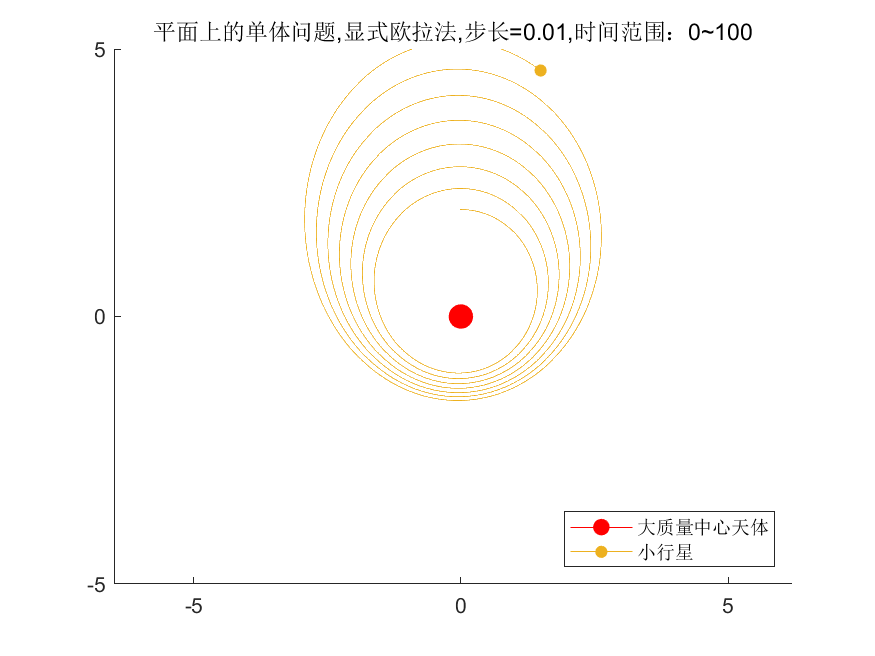
\includegraphics[width=0.45\textwidth]{各种方法的轨道形态对比//平面上的单体问题,显式欧拉法,步长=0.01,时间范围:0~100}}
	\subfigure[步长h=0.001]{
		\label{exEulr.sub.2}
		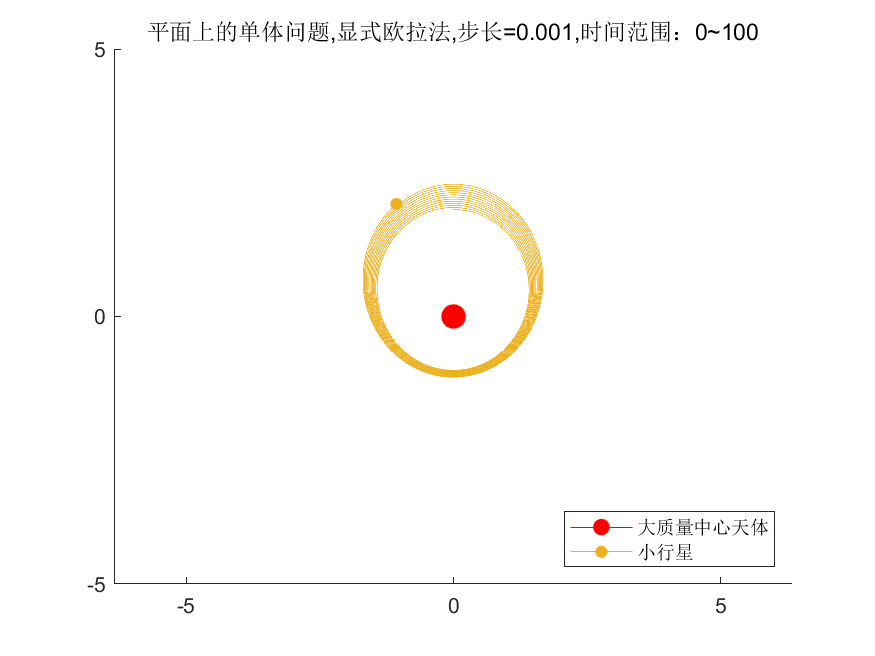
\includegraphics[width=0.45\textwidth]{各种方法的轨道形态对比//平面上的单体问题,显式欧拉法,步长=0.001,时间范围:0~100}}
	\caption{显式欧拉法}
	\label{exEuler.main}
\end{figure}
\par 图\ref{exEuler.sub.1}中可以发现轨道呈螺旋状向外发散。但是,在单体问题中,轨道的形状只可能是圆锥曲线(椭圆、抛物线、双曲线)的其中一种,不可能螺旋状发散。即便减小步长,图\ref{exEulr.sub.2}仍然可以看到轨道具有明显的螺旋状发散现象。可以认为,显式欧拉法对于求解N体问题不是一个好的方法。

\subsubsection{隐式欧拉法} 
\par 迭代格式:
$$
Y_{i+1} = Y_i + hf(t_{i+1},Y_{i+1})$$
\par 这是一个关于未知向量$Y_{i+1}$的非线性方程组,记$Y=Y_{i+1}$,需要使用高维牛顿法求解方程$F(Y)=0$。设置停止准则为$||F(Y)||<\text{1e-14}$,求得的运行轨迹如图\ref{imEuler.main}所示:
\begin{figure}[H]
	\centering  %图片全局居中
	\subfigure[步长h=0.01]{
		\label{imEuler.sub.1}
		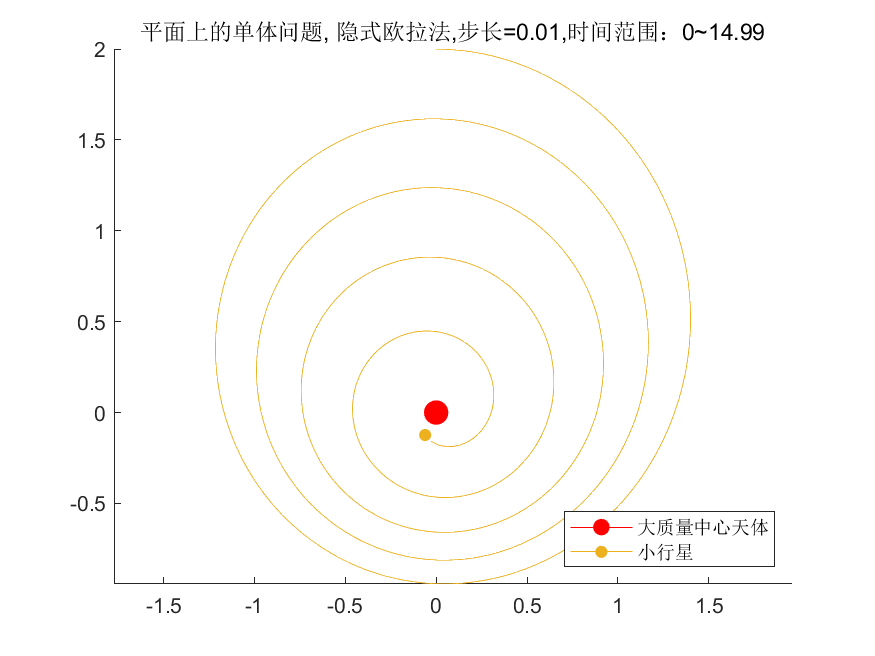
\includegraphics[width=0.45\textwidth]{各种方法的轨道形态对比//平面上的单体问题, 隐式欧拉法,步长=0.01,时间范围:0~14.99}}
	\subfigure[步长h=0.001]{
		\label{imEulr.sub.2}
		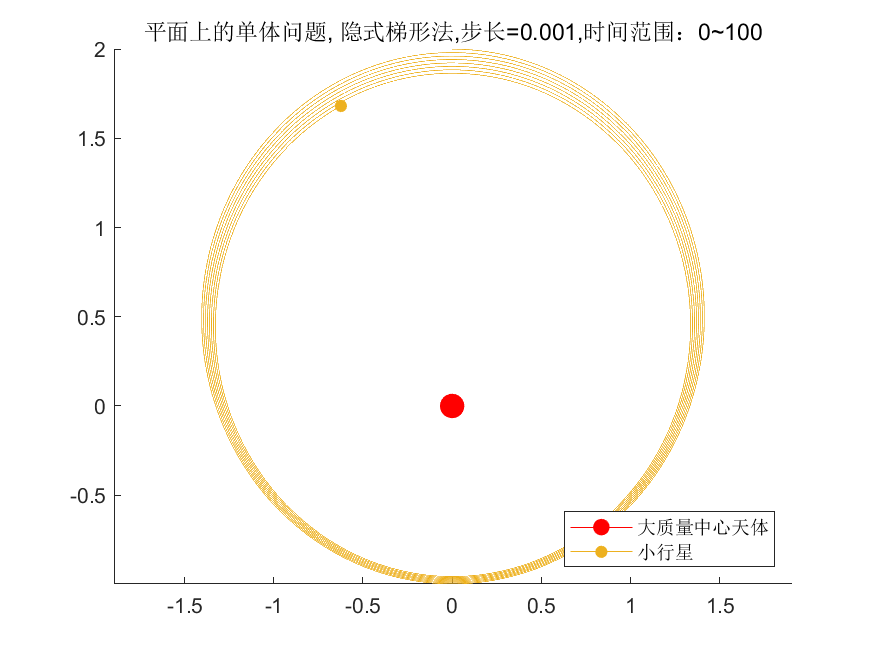
\includegraphics[width=0.45\textwidth]{各种方法的轨道形态对比//平面上的单体问题, 隐式梯形法,步长=0.001,时间范围:0~100}}
	\caption{隐式欧拉法}
	\label{imEuler.main}
\end{figure}
\par 图\ref{imEuler.sub.1}中观察到轨道呈螺旋状向中心收缩,这同样是不可能的。即便减少步长,当时间较长时,在图\ref{imEulr.sub.2}也可以观察到明显的收缩。因此,隐式欧拉法对于求解N体问题也不是一个好的方法。

\subsubsection{显式梯形法}
迭代格式:
$$
Y_{i+1} = Y_i + \frac{h}{2}(f(t_i,Y_i) + f( t_{i+1},Y_i+hf(t_i,Y_i)))$$
\par 统一设置步长$h=0.01$,显式梯形法的实验结果如图\ref{exTrap.main}所示,
\begin{figure}[H]
	\centering  %图片全局居中
	\subfigure[截至时间t=100]{
		\label{exTrap.sub.1}
		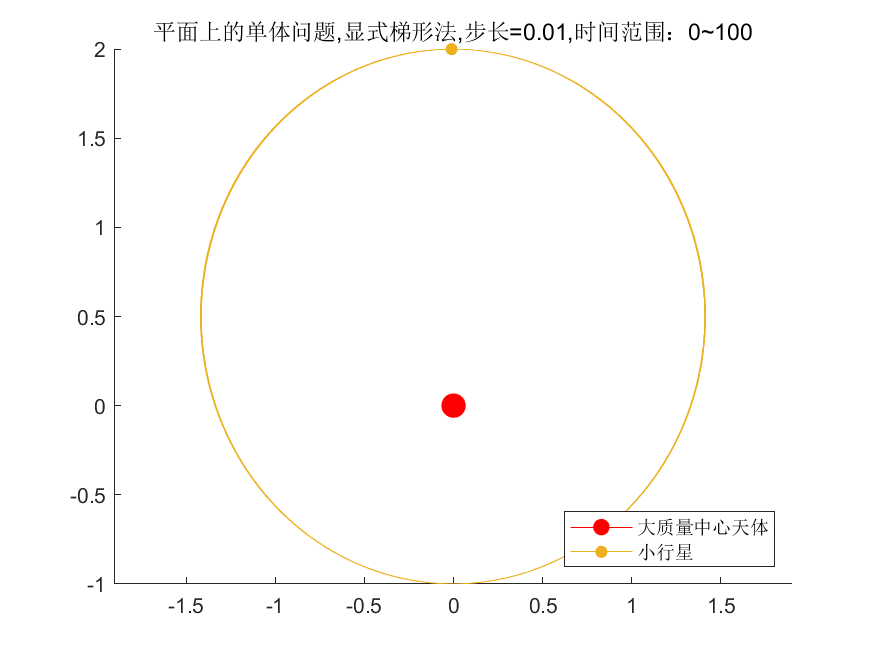
\includegraphics[width=0.3\textwidth]{各种方法的轨道形态对比//平面上的单体问题,显式梯形法,步长=0.01,时间范围:0~100}}
	\subfigure[截至时间t=1000]{
		\label{exTrap.sub.2}
		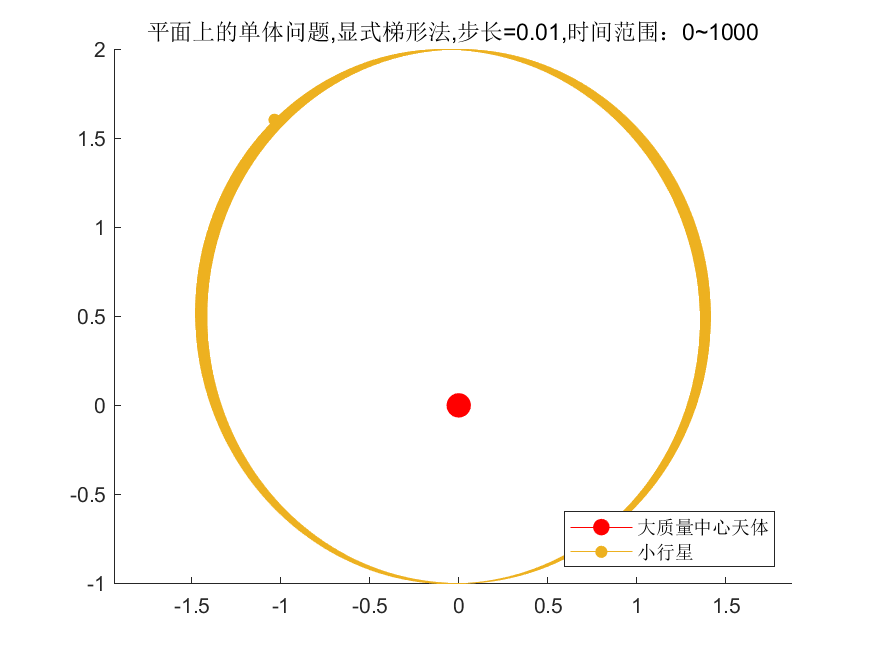
\includegraphics[width=0.3\textwidth]{各种方法的轨道形态对比//平面上的单体问题,显式梯形法,步长=0.01,时间范围:0~1000}}
	\subfigure[截至时间t=2000]{
		\label{exTrap.sub.3}
		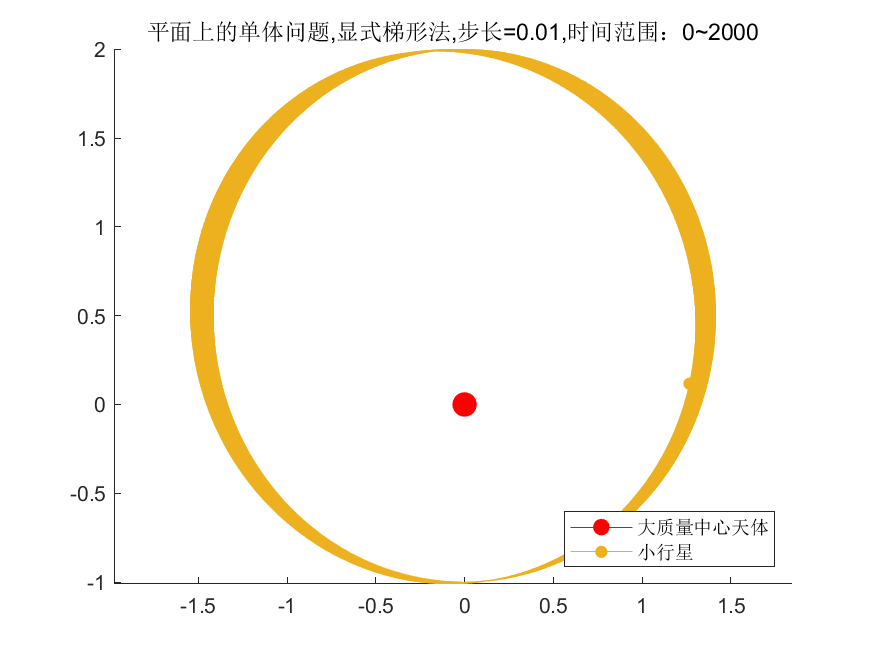
\includegraphics[width=0.3\textwidth]{各种方法的轨道形态对比//平面上的单体问题,显式梯形法,步长=0.01,时间范围:0~2000}}
	\caption{显式梯形法}
	\label{exTrap.main}
\end{figure}
可以看到,即便在时间比较长的情况下,与欧拉法相比,显示梯形法的轨道并没有呈现出向外发散或者向中心收敛的趋势。但精确性略差,能看到时间较长时轨迹出现偏移。

\subsubsection{隐式梯形法} 
\par 迭代格式:
$$
Y_{i+1} = Y_i + \frac{h}{2}(f(t_i,Y_i) + f(t_{i+1},Y_{i+1}))
$$
\par 这是一个关于未知向量$Y_{i+1}$的非线性方程组,记$Y=Y_{i+1}$,需要使用高维牛顿法求解方程$H(Y)=0$。同样设置停止准则为$||H(Y)||<\text{1e-14}$,求得的运行轨迹如图\ref{imEuler.main}所示:
\begin{figure}[H]
	\centering  %图片全局居中
	\subfigure[步长h=0.01]{
		\label{imTrap.sub.1}
		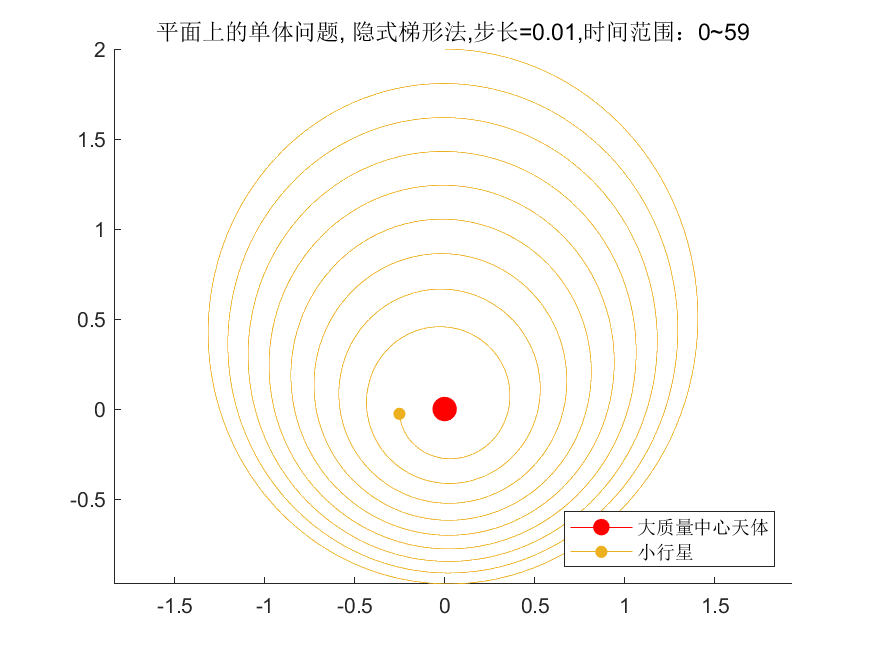
\includegraphics[width=0.45\textwidth]{各种方法的轨道形态对比//平面上的单体问题, 隐式梯形法,步长=0.01,时间范围:0~59}}
	\subfigure[步长h=0.001]{
		\label{imTrap.sub.2}
		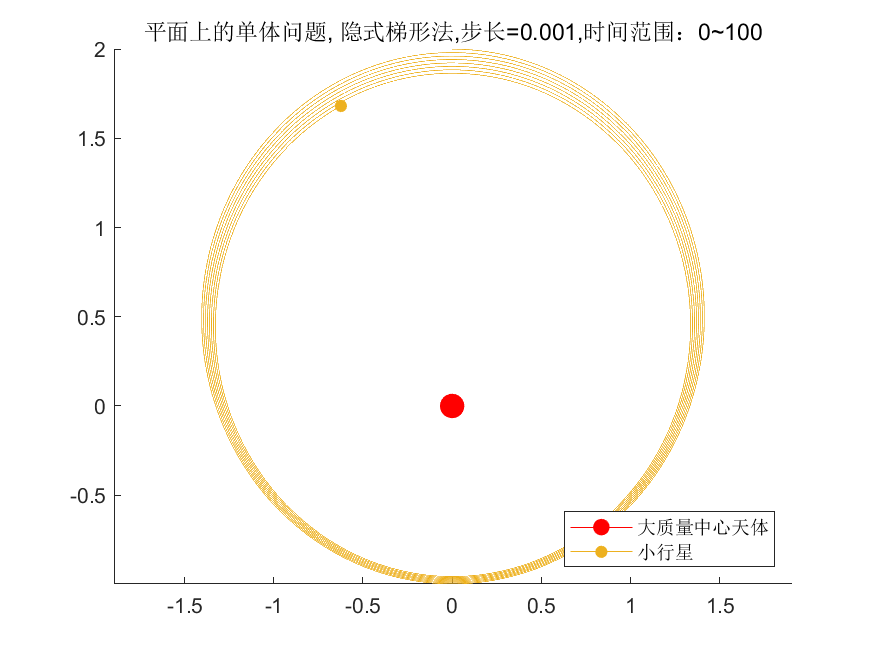
\includegraphics[width=0.45\textwidth]{各种方法的轨道形态对比//平面上的单体问题, 隐式梯形法,步长=0.001,时间范围:0~100}}
	\caption{隐式梯形法}
	\label{imTrap.main}
\end{figure}
\par 图\ref{imTrap.sub.1}中观察到轨道呈螺旋状向中心收缩,即便减少步长,当时间较长时,在图\ref{imTrap.sub.2}也可以观察到明显的收缩趋势。因此,隐式梯形法对于求解N体问题而言并不是一个好的方法。

\subsubsection{Störmer-Verlet}
\par 对SV方法的分析可参见文献\cite{gardarsson2013some},SV对于力学类的问题特别适用。该方法的迭代方式比较特别,需要特殊说明。设位置向量$r=[x,y]$,速度向量$v=[v_x,v_y]$,SV首先让速度向量v走“半步”:
$$v_{1/2} = v_0 + \frac{h}{2}a(r_0)$$
\par 然后r和v交错地迭代:
$$r_{k+1} = r_k + hv_{k+1/2}$$
$$v_{k+3/2} = v_{k+1/2} + ha(r_{k+1})$$
\par 其中$a(r)=[\frac{-Gmx}{d^3},\frac{-Gmy}{d^3}]^T$, $d=\sqrt{x^2+y^2}$ 
\par 实验结果如下。
\begin{figure}[H]
	\centering  %图片全局居中
	\subfigure[截至时间t=100]{
		\label{sv.sub.1}
		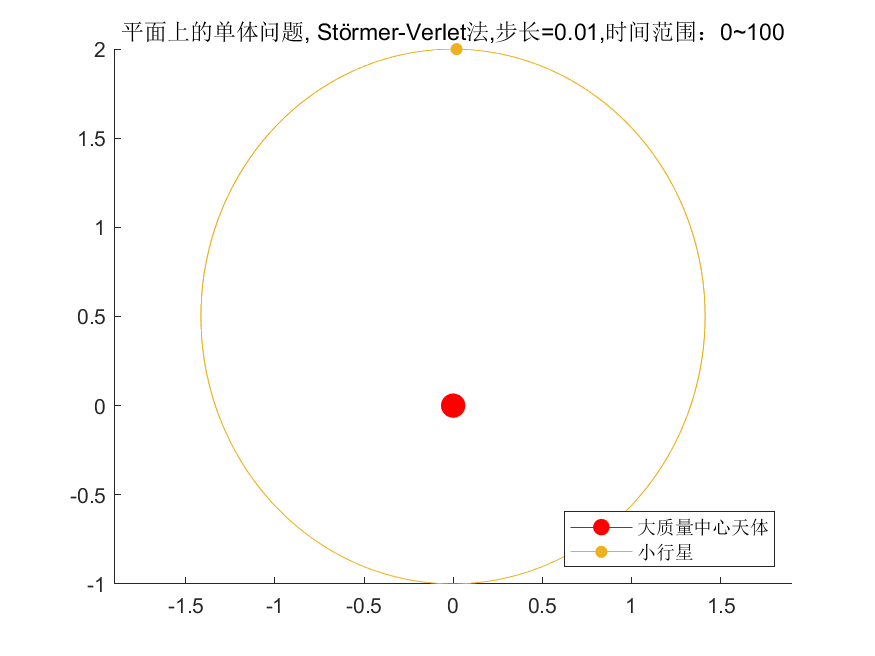
\includegraphics[width=0.3\textwidth]{各种方法的轨道形态对比//平面上的单体问题, Störmer-Verlet法,步长=0.01,时间范围:0~100}}
	\subfigure[截至时间t=1000]{
		\label{sv.sub.2}
		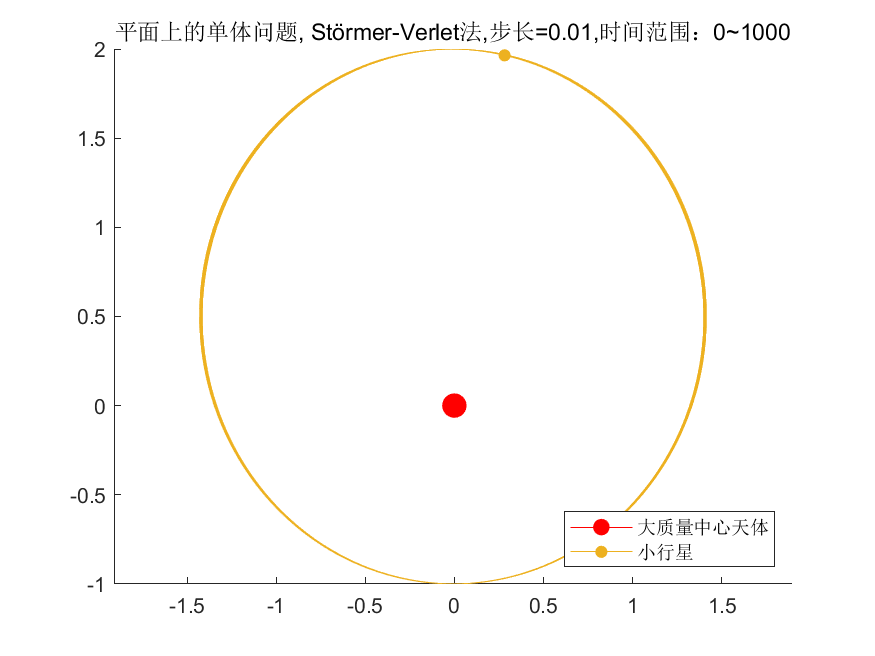
\includegraphics[width=0.3\textwidth]{各种方法的轨道形态对比//平面上的单体问题, Störmer-Verlet法,步长=0.01,时间范围:0~1000}}
	\subfigure[截至时间t=2000]{
		\label{sv.sub.3}
		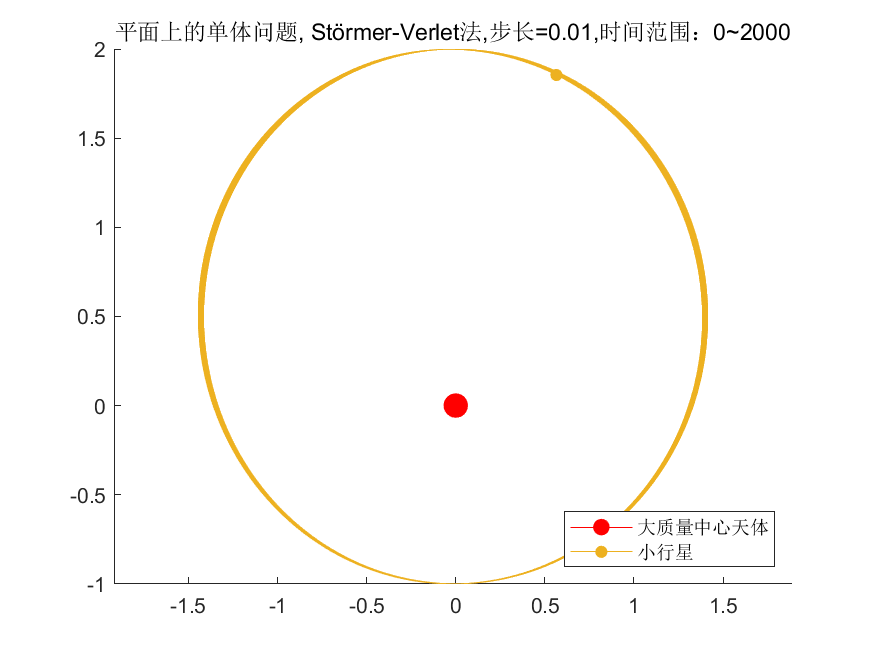
\includegraphics[width=0.3\textwidth]{各种方法的轨道形态对比//平面上的单体问题, Störmer-Verlet法,步长=0.01,时间范围:0~2000}}
	\caption{SV方法}
	\label{sv.main}
\end{figure}
\par 对比图\ref{exTrap.main}和图\ref{sv.main},SV方法计算的轨道比显示梯形法更加精确。

\subsubsection{RK4}
\par 这是龙格-库塔系列中最为经典的方法,基本迭代格式如下:
\begin{align*}
	Y_{i+1} &= Y_i + \frac{h}{6}(s_1+2s_2+2s_3+s4)\\
	s1 &= f(t_i,Y_i)\\
	s2 &= f(t_i+\frac{h}{2},Y_i+\frac{h}{2}s_1)\\
	s3 &= f(t_i+\frac{h}{2},Y_i+\frac{h}{2}s_2)\\
	s4 &= f(t_i+h,Y_i+hs_3)
\end{align*}
\par 实验结果如下图所示
\begin{figure}[H]
	\centering  %图片全局居中
	\subfigure[截至时间t=100]{
		\label{rk4.sub.1}
		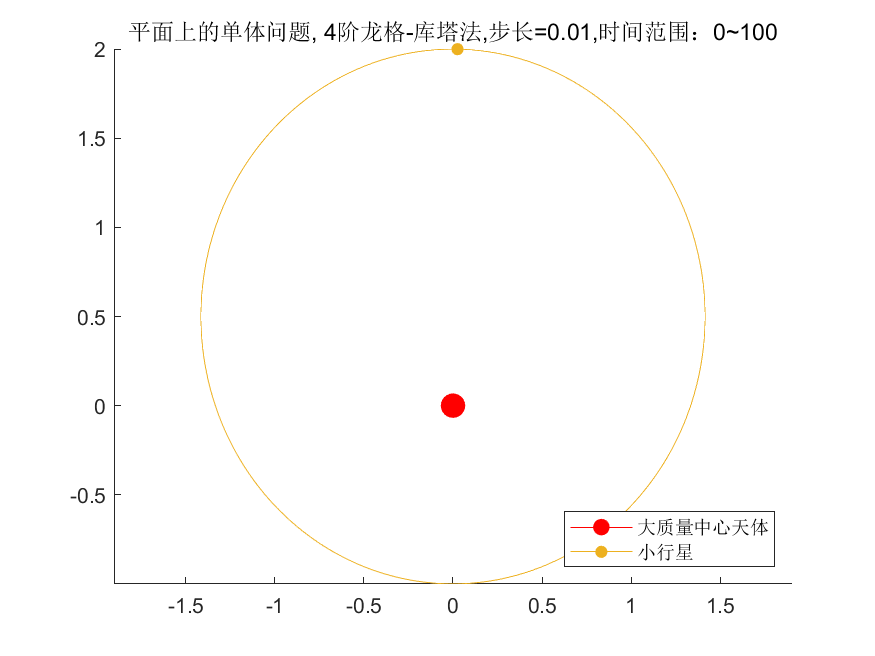
\includegraphics[width=0.3\textwidth]{各种方法的轨道形态对比//平面上的单体问题, 4阶龙格-库塔法,步长=0.01,时间范围:0~100}}
	\subfigure[截至时间t=1000]{
		\label{rk4.sub.2}
		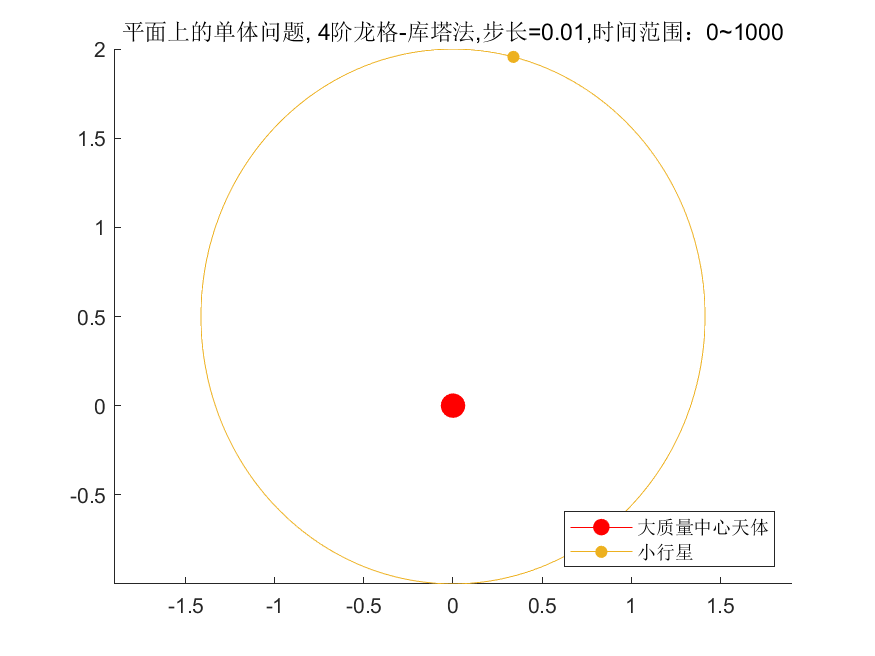
\includegraphics[width=0.3\textwidth]{各种方法的轨道形态对比//平面上的单体问题, 4阶龙格-库塔法,步长=0.01,时间范围:0~1000}}
	\subfigure[截至时间t=2000]{
		\label{rk4.sub.3}
		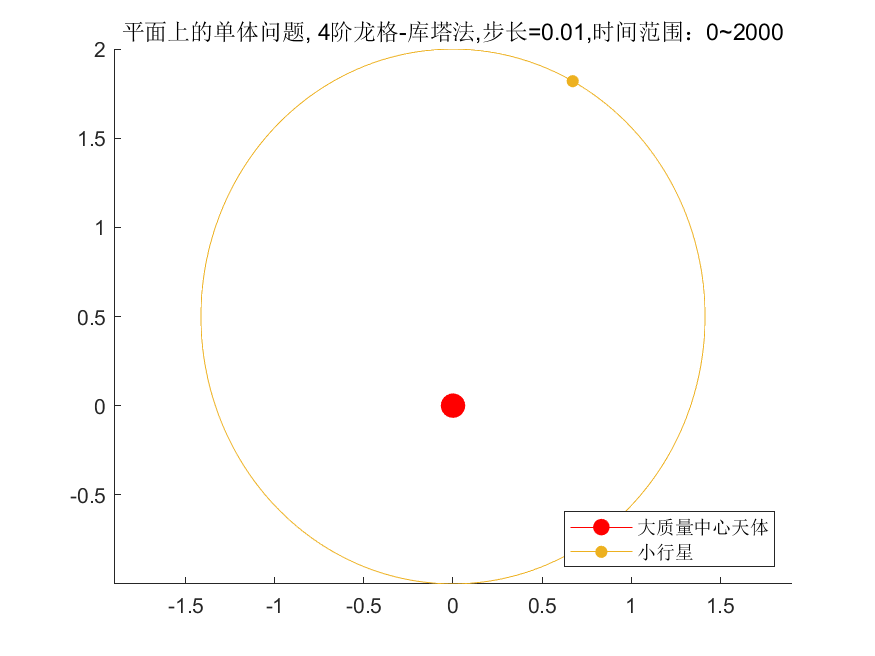
\includegraphics[width=0.3\textwidth]{各种方法的轨道形态对比//平面上的单体问题, 4阶龙格-库塔法,步长=0.01,时间范围:0~2000}}
	\caption{SV方法}
	\label{rk4.main}
\end{figure}
\par 对比图\ref{exTrap.main},图\ref{sv.main}和图\ref{rk4.main}可以看出,在较长时间的情况下,RK4计算的轨道精确性仍然很高。
\par 在以上实验中可以看出,显式梯形法、SV法和RK4的精确性都较高。接下来将探索他们全局误差的阶数。

\subsection{显式梯形法,SV和RK4的全局误差}
\par 在接下来的单体问题实验中,设置中心天体的质量为$4\pi^2$,设置小行星的初始条件为:
$${x=0}, {v_x=2\pi}, {y=1},{v_y=0}$$
\par 此时单体运动的轨迹是圆轨道,周期为T=1。分别计算显式梯形法、SV、RK4三种方法在t=10(也即十个周期后,理论上应该回到起点)的位置到起点处$(0,1)$的欧氏距离作为全局误差,并观察全局误差随h的变化情况,做出双对数图\ref{globalError}如下:
\begin{figure}[H]
	\centering  %图片全局居中
	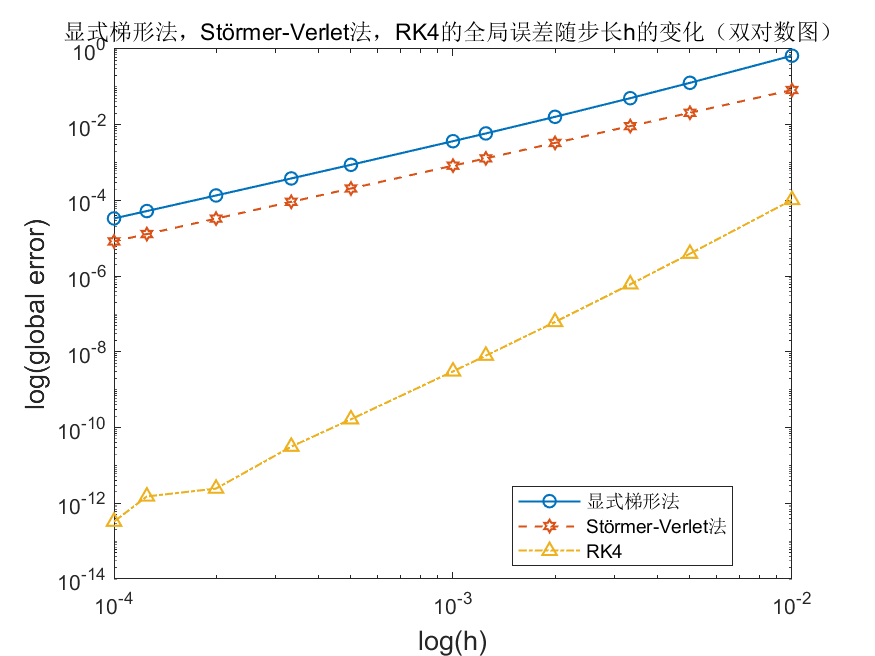
\includegraphics[width=0.7\textwidth]{圆轨道-轨道误差//三种方法的全局误差随步长h的变化(双对数图)}
	\caption{三种数值方法的全局误差随步长h的变化(双对数图)}
	\label{globalError}
\end{figure}
\par 观察三种方法在双对数图中的斜率可以知道,显式梯形法和RK4的收敛阶都为$O(h^2)$,RK4的收敛阶为$O(h^4)$,并且SV法的误差比显示梯形法更小。

\subsection{显式梯形法,SV和RK4的机械能变化}
\par 最后,我们再比较三种方法的机械能变化情况。接下来统一使用二体问题进行测试。初始状态(该初始状态借鉴于参考文献\cite{sauer2018数值分析})为:
\begin{align*}
	m_1&=0.3,x_1=2,y_1=2,v_{x_1}=0.2,v_{y_1}=-0.2;\\
	m_2&=0.03,x_2=0,y_2=0,v_{x2}=-0.01,v_{y2}=0.01;
\end{align*}

\par 这种初始条件下,会形成双星系统,轨迹大致如下:
\begin{figure}[H]
	\centering  %图片全局居中
	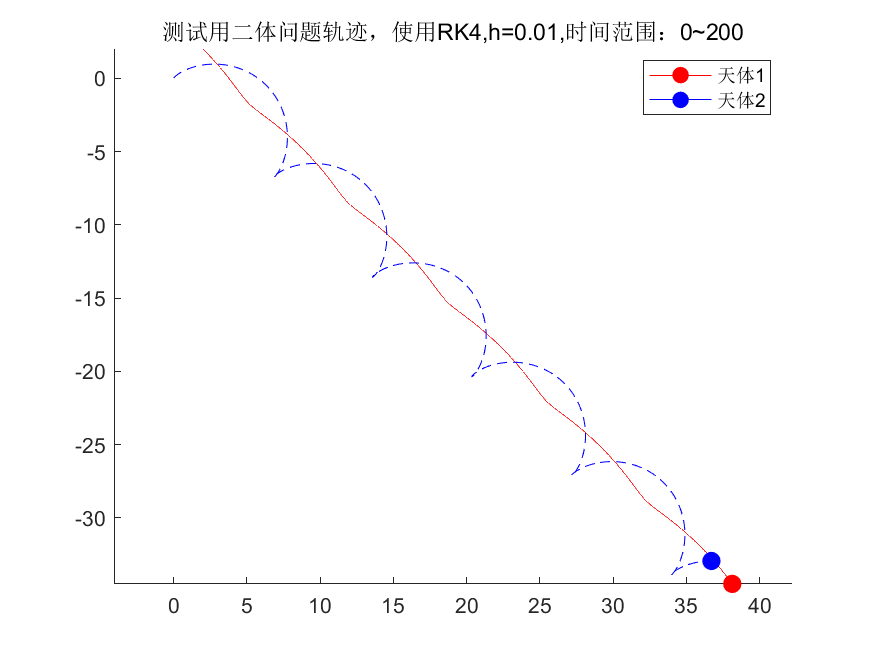
\includegraphics[width=0.7\textwidth]{二体问题-能量误差//测试用二体问题轨迹,使用RK4,h=0.01,时间范围:0~200}
	\caption{测试用的二体问题轨迹}
	\label{Two-Body-orbit}
\end{figure}
\par 显式梯形法的机械能变化情况如下,可以看出,随着时间的增加,显式梯形法计算的二体系统机械能呈现上升趋势。:
\begin{figure}[H]
	\centering  %图片全局居中
	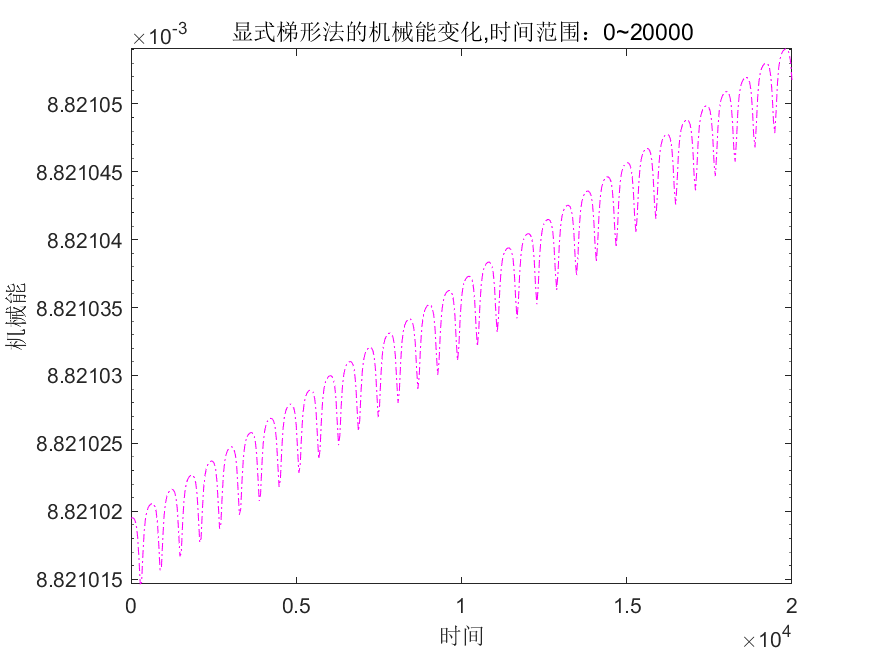
\includegraphics[width=0.7\textwidth]{二体问题-能量误差//显式梯形法的机械能变化,时间范围:0~20000}
	\caption{显式梯形法的机械能变化情况(每隔4000步记录一次机械能)}
	\label{Two-Body-energy-exTrap}
\end{figure}

\par RK4的机械能变化情况如下,和显式梯形法相比,RK4计算的二体系统的机械能的波动的范围相当地小,且整体上看不出明显的上升或下降趋势:
\begin{figure}[H]
	\centering  %图片全局居中
	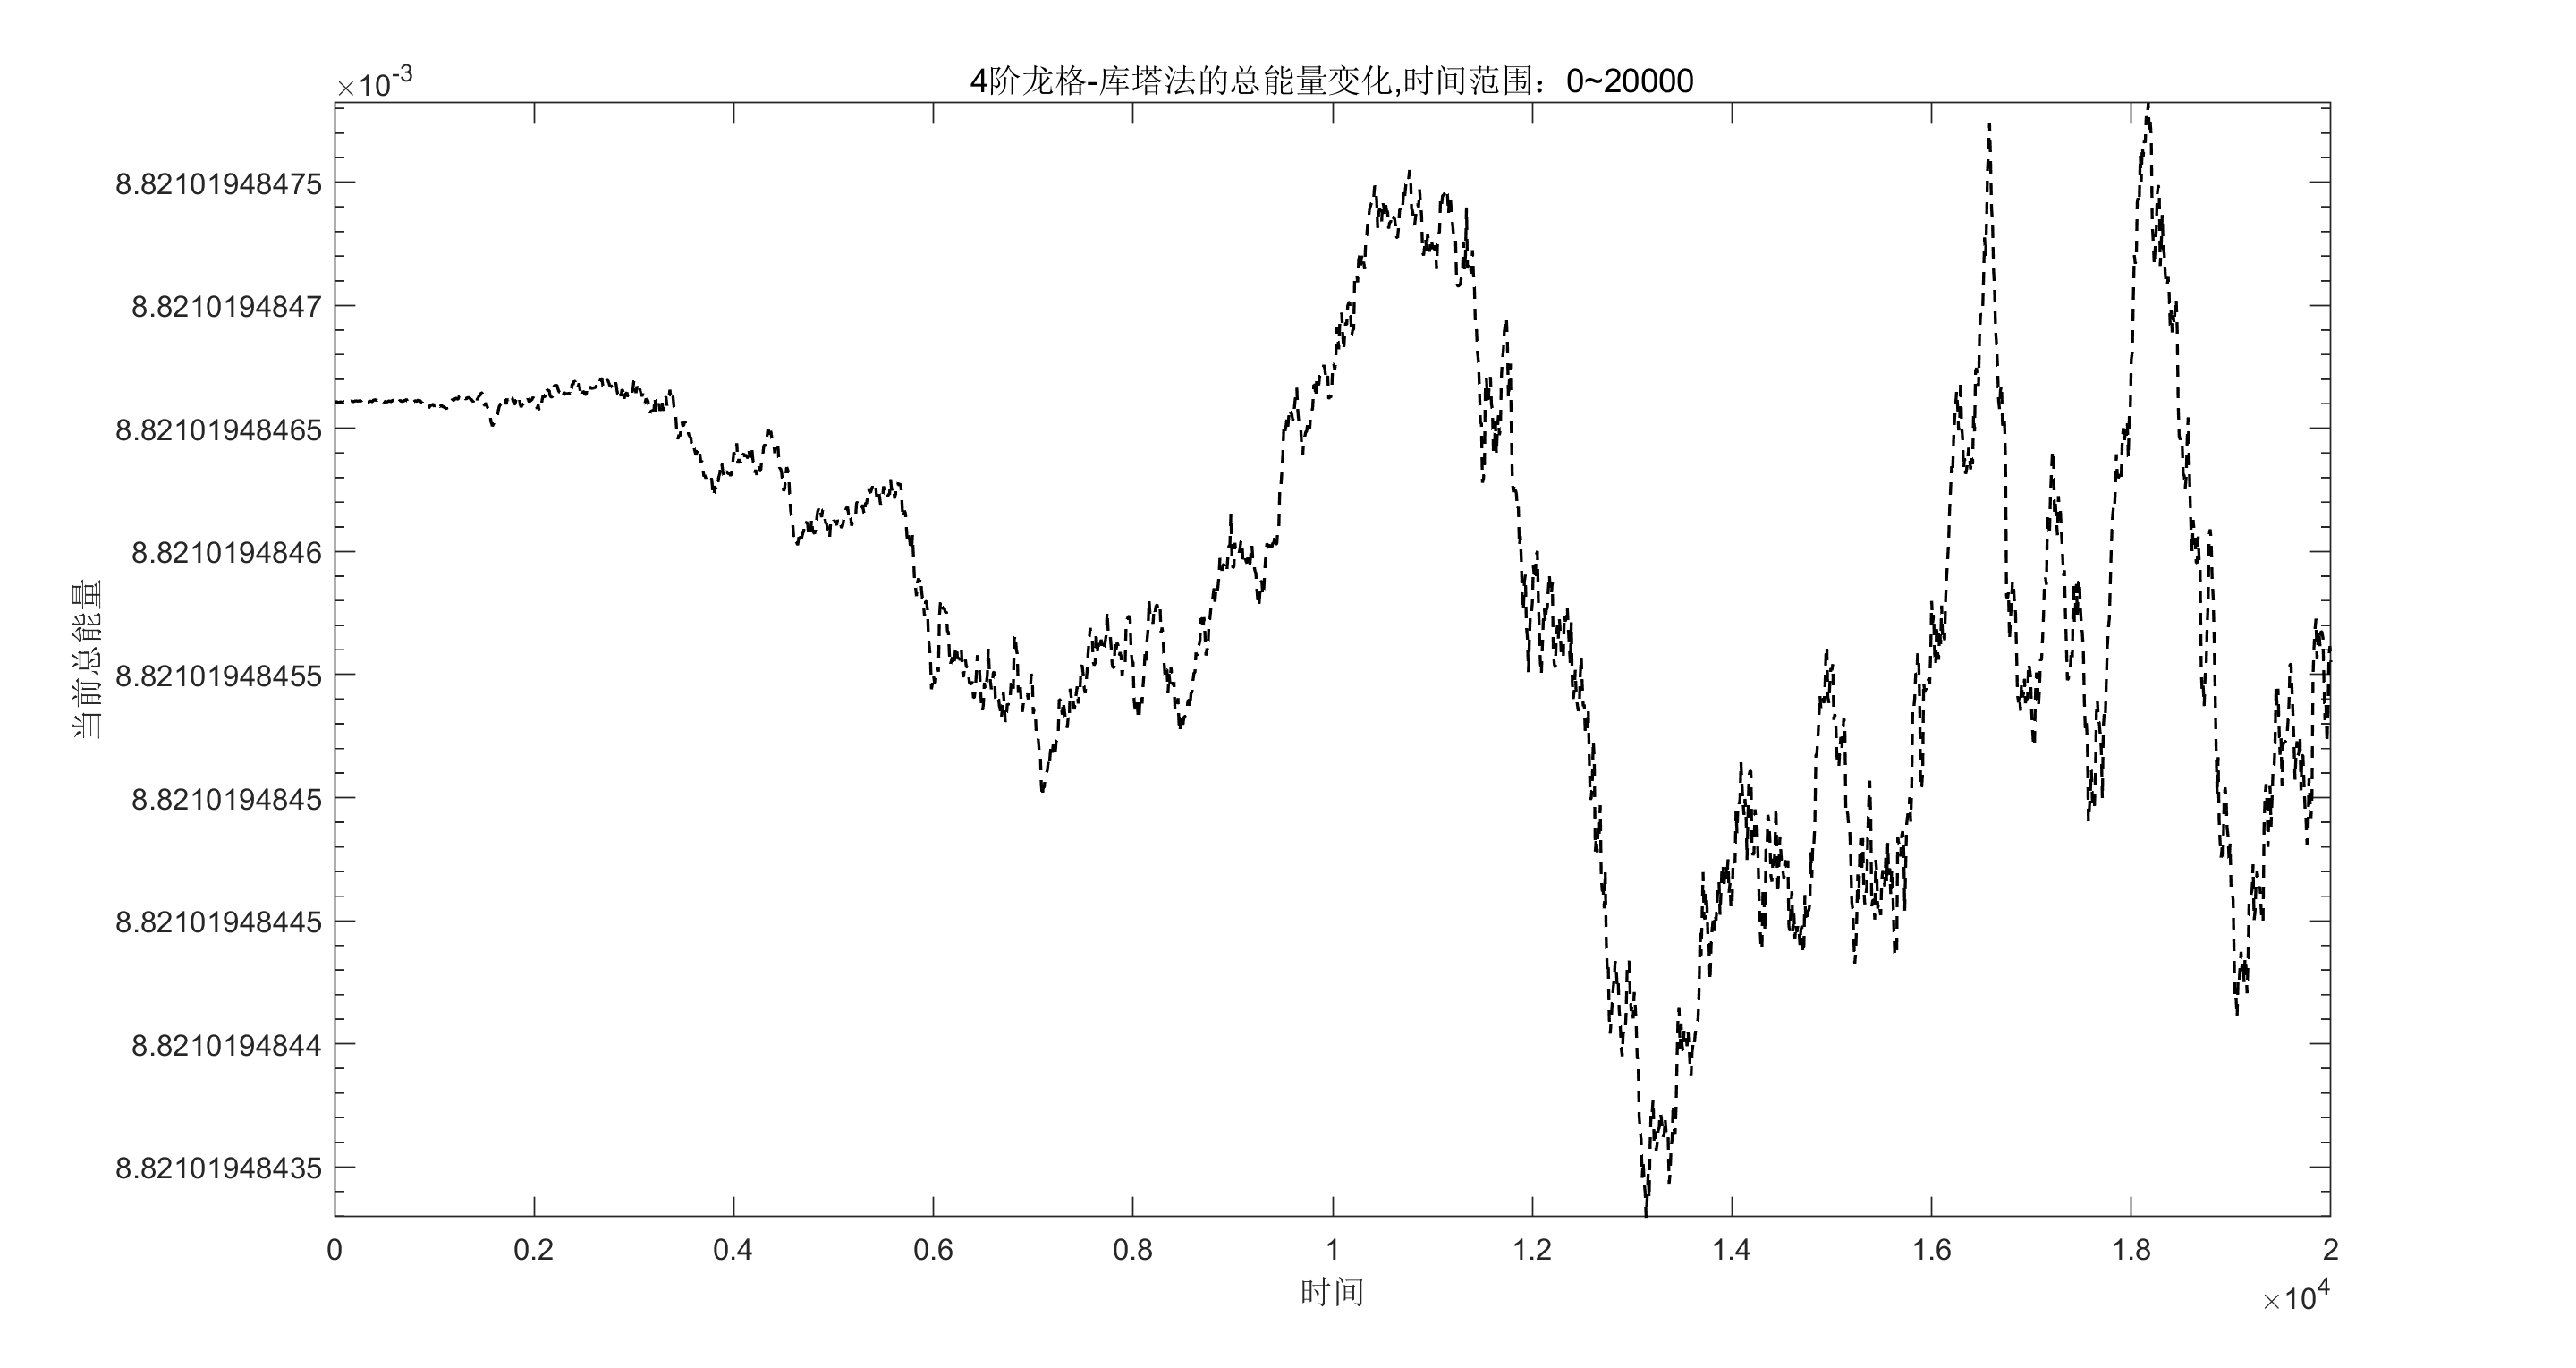
\includegraphics[width=0.7\textwidth]{二体问题-能量误差//4阶龙格-库塔法的总能量变化,时间范围:0~20000}
	\caption{RK4的机械能变化情况(每隔1000步记录一次机械能)}
	\label{Two-Body-energy-RK4}
\end{figure}
 
\par SV的机械能无法直接计算,因为无法获得同一时刻两个天体的位置和速度,但这又是计算机械能所必须的。那么,只好分别使用使用$r_k$和$v_{k+1/2}$进行近似,计算机械能变化情况如下:
\begin{figure}[H]
	\centering  %图片全局居中
	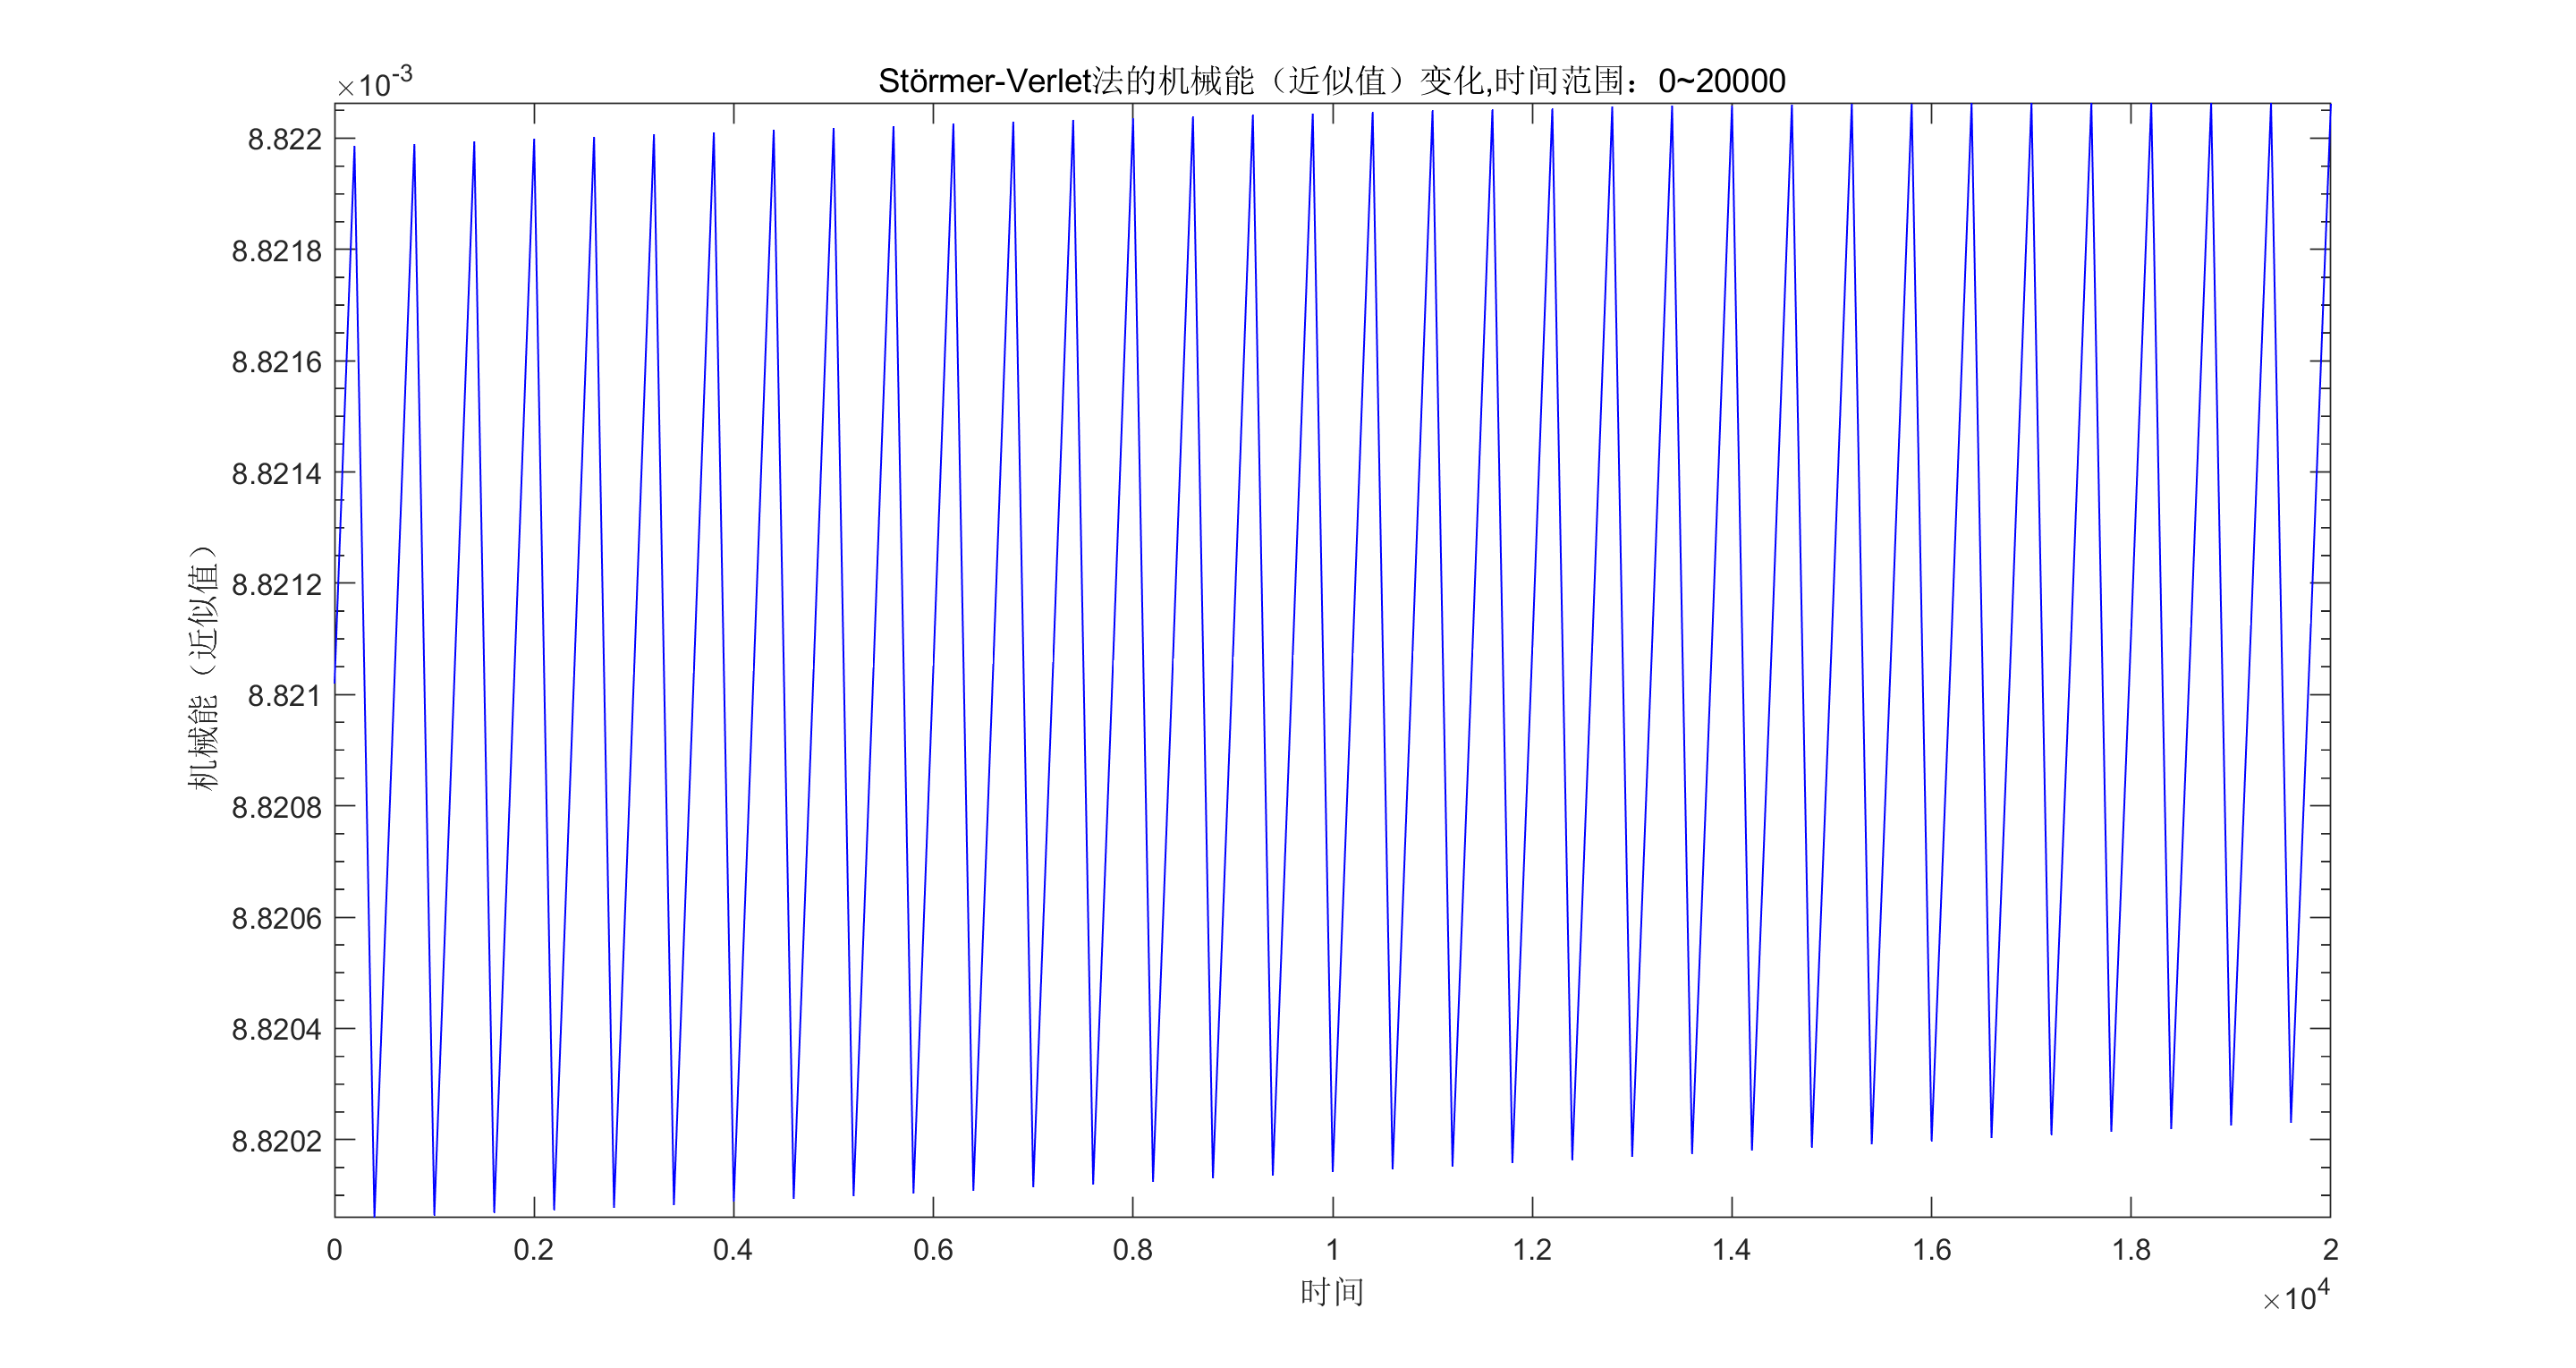
\includegraphics[width=0.7\textwidth]{二体问题-能量误差//Störmer-Verlet法的机械能(近似值)变化,时间范围:0~20000}
	\caption{SV的“近似”机械能变化情况(每隔20000步记录一次机械能)}
	\label{Two-Body-energy-SV}
\end{figure}
\par 观察到SV的机械能呈现剧烈震动的特点,出现这种现象的可能原因是:这只是“近似的机械能”。即便是“近似的”机械能,观察其震动的峰值的变化,可以推测SV方法计算的二体系统的机械能也有略微上升的趋势。
\par 
\par 小结:在计算N体问题时,多种方法中,显式梯形法、SV和RK4计算的运动轨道比较精确。显式梯形法和SV法为2阶收敛,RK4为4阶收敛。显式梯形法和SV计算得到的系统机械能会呈现上升趋势,而RK4计算得到的系统机械能则相对稳定,没有明显的上升或下降趋势。在本文的后续部分,如无特殊说明,都默认使用最为精确的RK4进行数值模拟。

\section{几种具有代表性的周期性轨道}
\par 在没有给定特殊初始条件下,三体问题的轨迹往往呈现混乱、无规律的状态,十分常见的一种情况是,两个天体形成双星系统,而第三个天体被向外抛射到无穷远。这些无规律的情况并不是本节所主要关心的。本节将首先展示一些具有代表性的三体运动的周期性轨道,然后用八字轨道和毕达哥拉斯问题展示三体问题对初值敏感的特点。

\par 目前已发现的周期性轨道基本都收录在这个网站\url{http://three-body.ipb.ac.rs}。本文从该网站中选择了一部分具有代表性的轨道进行测试。统一设置$G=1,m_1=m_2=m_3=1$,实验结果如下。
\subsection{Broucke R 1 }
\par 关于这个轨道的更多信息可参考\url{http://three-body.ipb.ac.rs/bsol.php?id=16}
\par 初始条件如下:
\begin{align*}
	x_1 &= 0.8083106230, y_1 = 0,
	v_{x_1} = 0, v_{y_1} = 0.9901979166; \\
	x_2 &= -0.4954148566, y_2 = 0,
	v_{x_2} = 0, v_{y_2} = -2.7171431768;\\ 
	x_3 &= -0.3128957664, y_3 = 0,
	v_{x_3} = 0, v_{y_3} = 1.7269452602;
\end{align*}
\par 轨迹如下:
\begin{figure}[H]
	\centering  %图片全局居中
	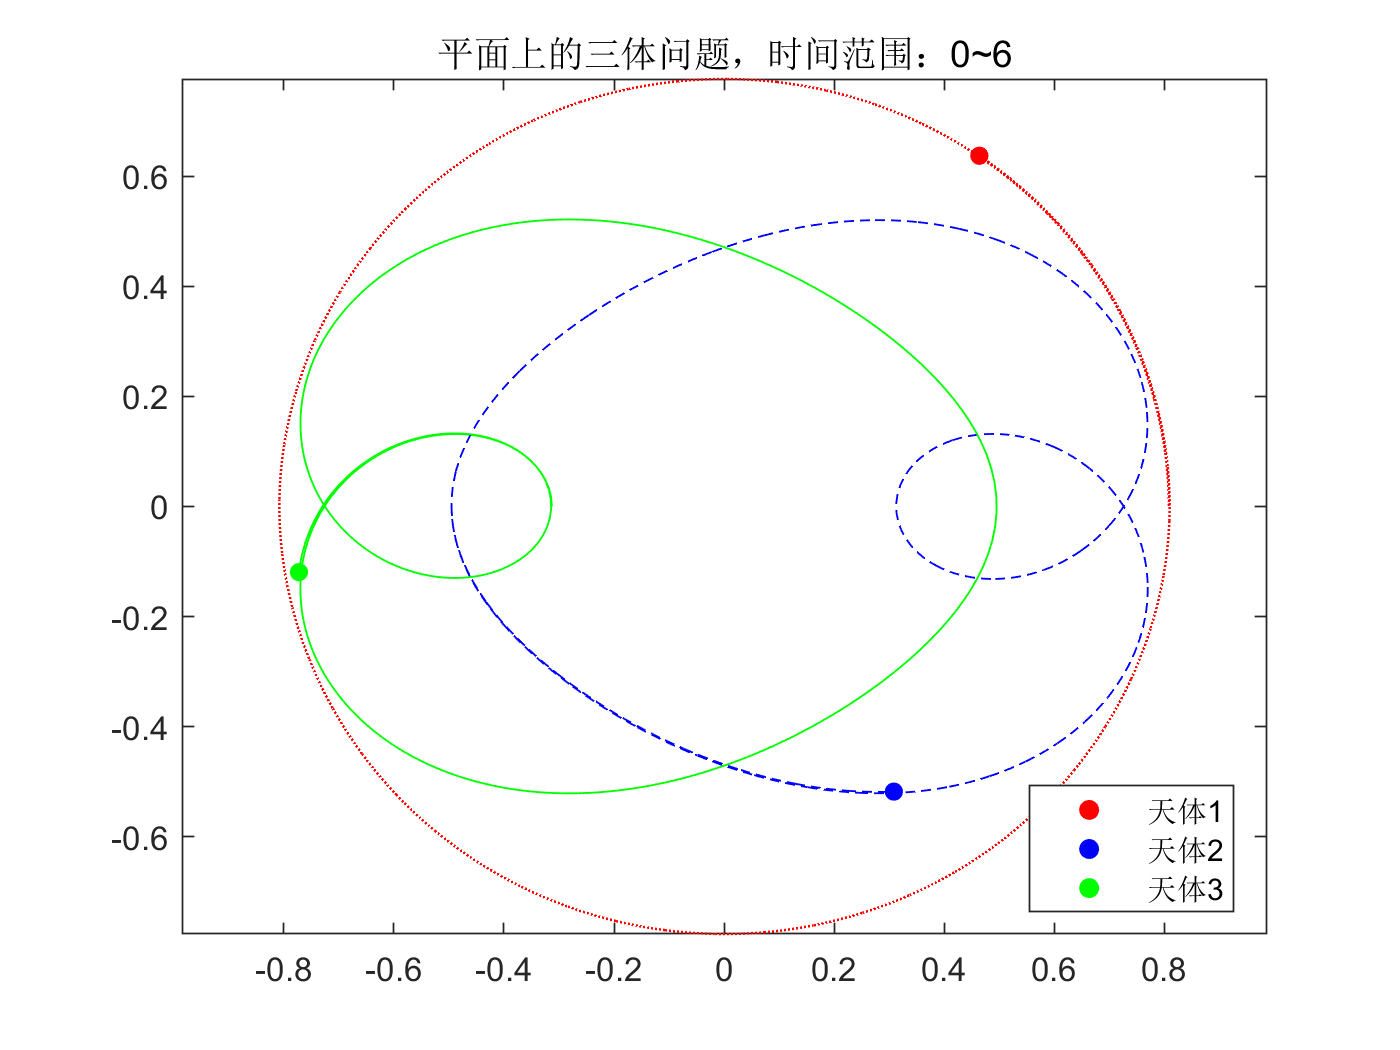
\includegraphics[width=0.7\textwidth]{一些优美的周期解//Broucke R 1}
	\caption{Broucke R 1的轨迹}
	\label{Broucke_R_1}
\end{figure}

\subsection{Henon 35}
\par 关于这个轨道的更多信息可参考\url{http://three-body.ipb.ac.rs/hsol.php?id=33}
\par 初始条件如下:
\begin{align*}
	x_1&= 0.0797756841 , y_1= 0,	v_{x_1}= 0, v_{y_1}= 1.1801414216;\\
	x_2&= 1.1140666180 , y_2= 0, 	v_{x_2}= 0, v_{y_2}= -0.2727205239;\\
	x_3&= -1.1938423022 ,y_3=0,		v_{x3}= 0, v_{y_3}= -0.9074208977;
\end{align*}
\par 轨迹如下:
\begin{figure}[H]
	\centering  %图片全局居中
	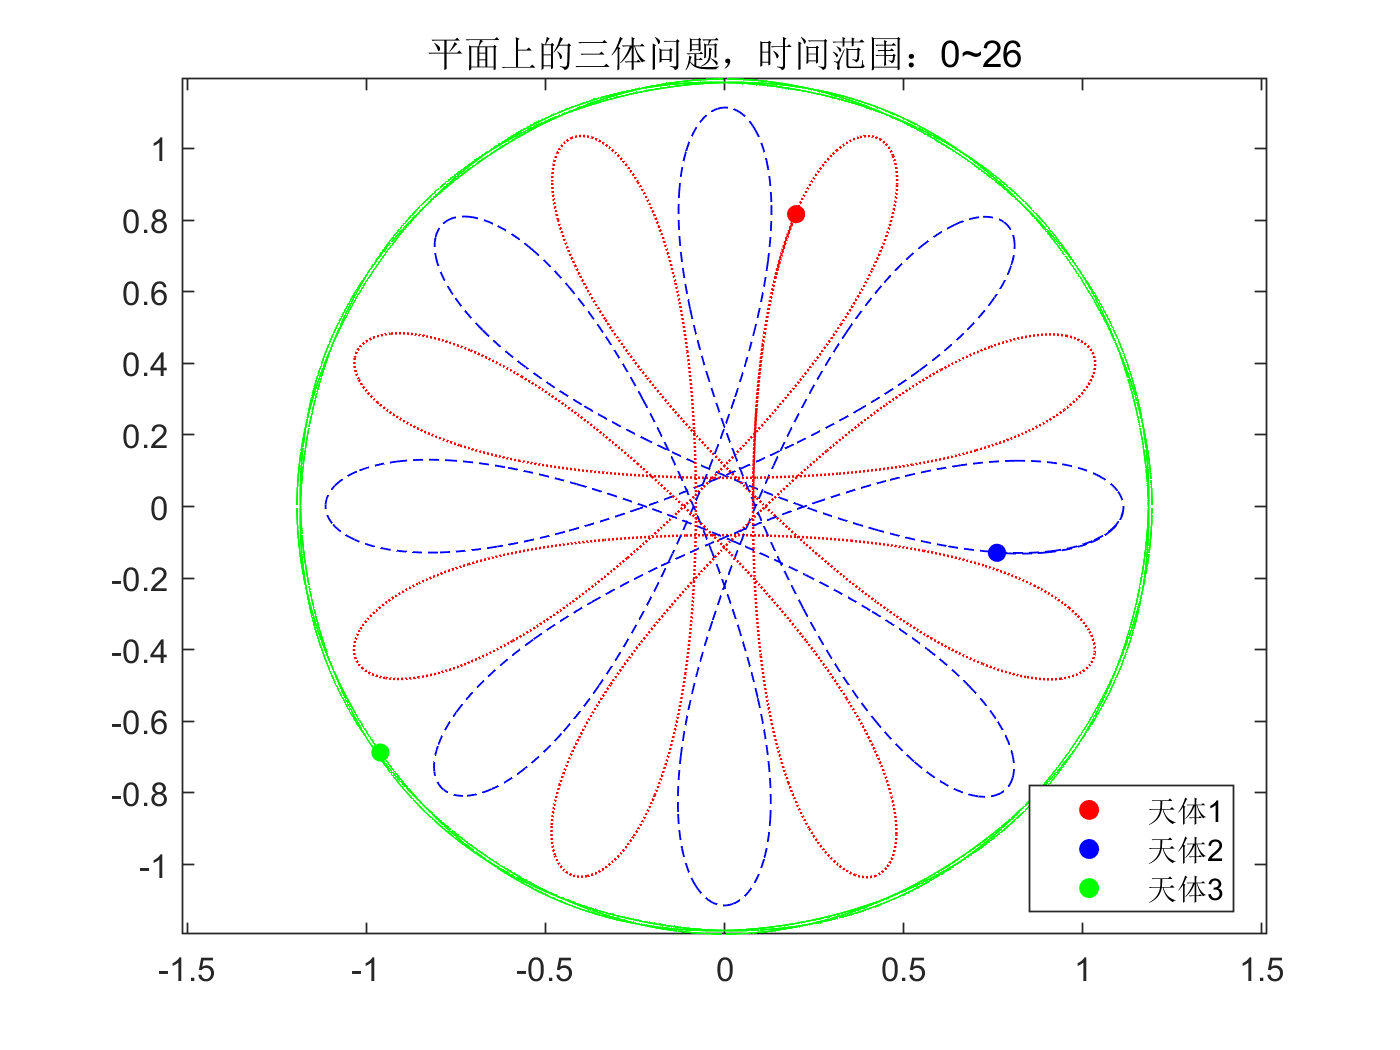
\includegraphics[width=0.7\textwidth]{一些优美的周期解//Henon 35}
	\caption{Henon 35的轨迹}
	\label{Henon_35}
\end{figure}

\subsection{Oval, catface, and starship}
\par
关于这个轨道的更多信息可参考\url{http://three-body.ipb.ac.rs/sheen_sol.php?id=1}
\par 初始条件如下:
\begin{align*}
	x_1&= 0.536387073390 ,y_1= 0.054088605008,v_{x_1}= -0.569379585581, v_{y_1}= 1.255291102531;\\
	x_2&= -0.252099126491 ,y_2= 0.694527327749,	v_{x_2}= 0.079644615252 ,v_{y_2}= -0.458625997341;\\
	x_3&= -0.275706601688 ,y_3=-0.335933589318,v_{x_3}= 0.489734970329, v_{y_3}= -0.796665105189;
\end{align*}
\par 轨迹如下:
\begin{figure}[H]
	\centering  %图片全局居中
	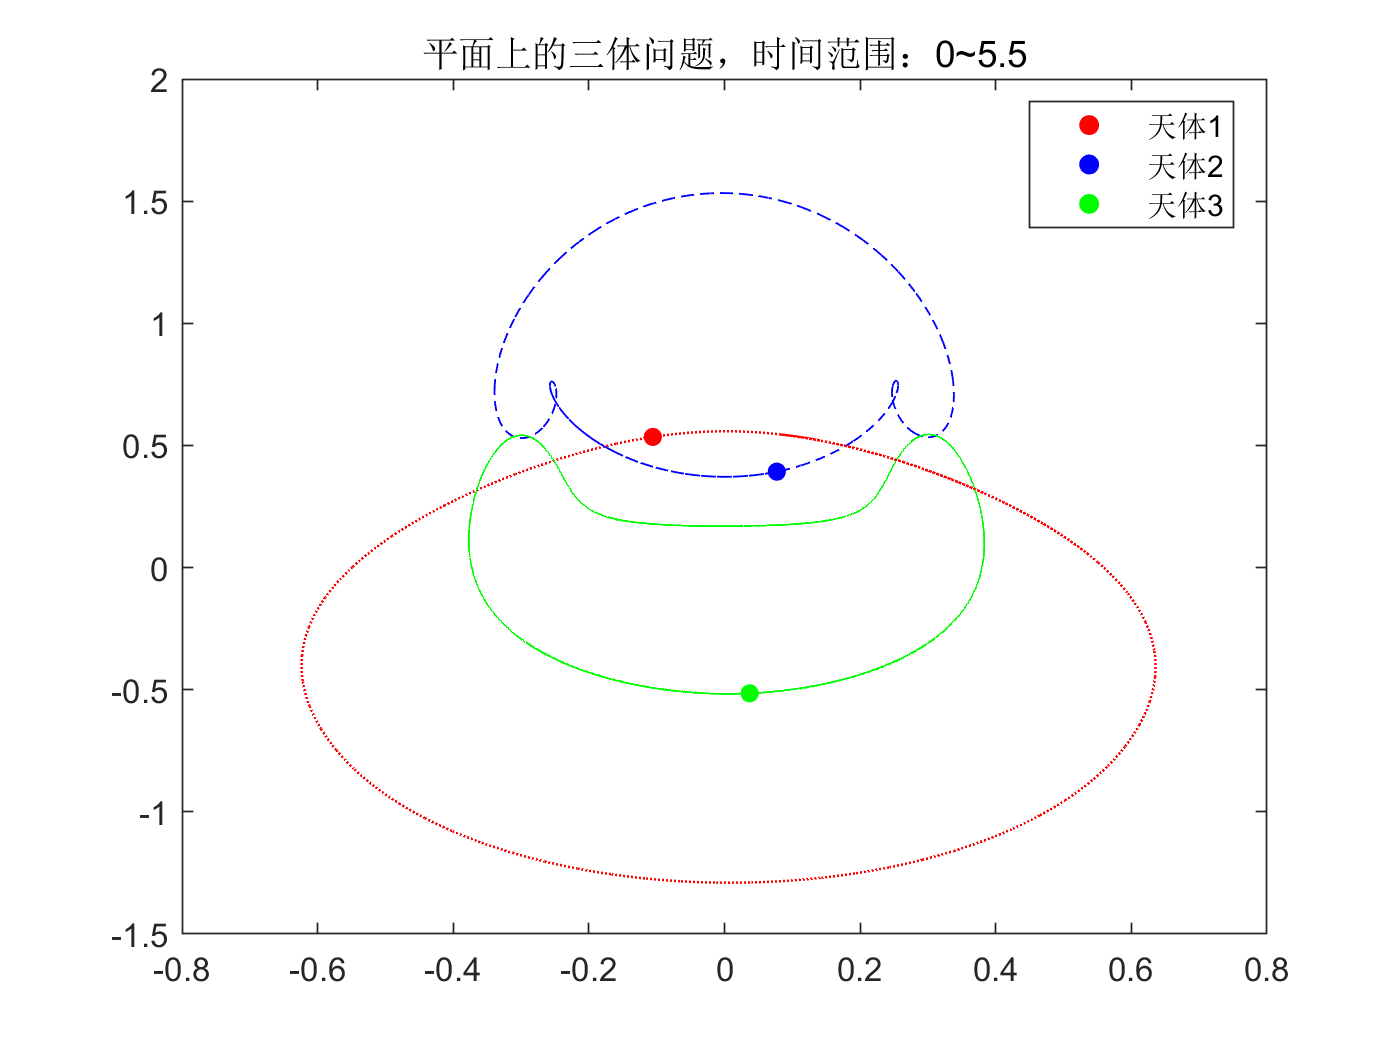
\includegraphics[width=0.7\textwidth]{一些优美的周期解//Oval, catface, and starship}
	\caption{Oval, catface, and starship的轨迹}
	\label{OCS}
\end{figure}

\subsection{GOGGLES}
\par
关于这个轨道的更多信息可参考\url{http://three-body.ipb.ac.rs/sol.php?id=6}

\par 初始条件如下:
\begin{align*}
	p_1 &= 0.083300, p_2= 0.127889;\\
	x_1&= -1 , y_1= 0,	v_{x_1}= p_1, v_{y_1}= p_2;\\
	x_2&= 1 , y_2= 0,	v_{x_2}= p_1, v_{y_2}= p_2;\\
	x_3&= 0 ,y_3=0,		v_{x3}= -2p_1; v_{y_3}= -2p_2;
\end{align*}
\par 轨迹如下:
\begin{figure}[H]
	\centering  %图片全局居中
	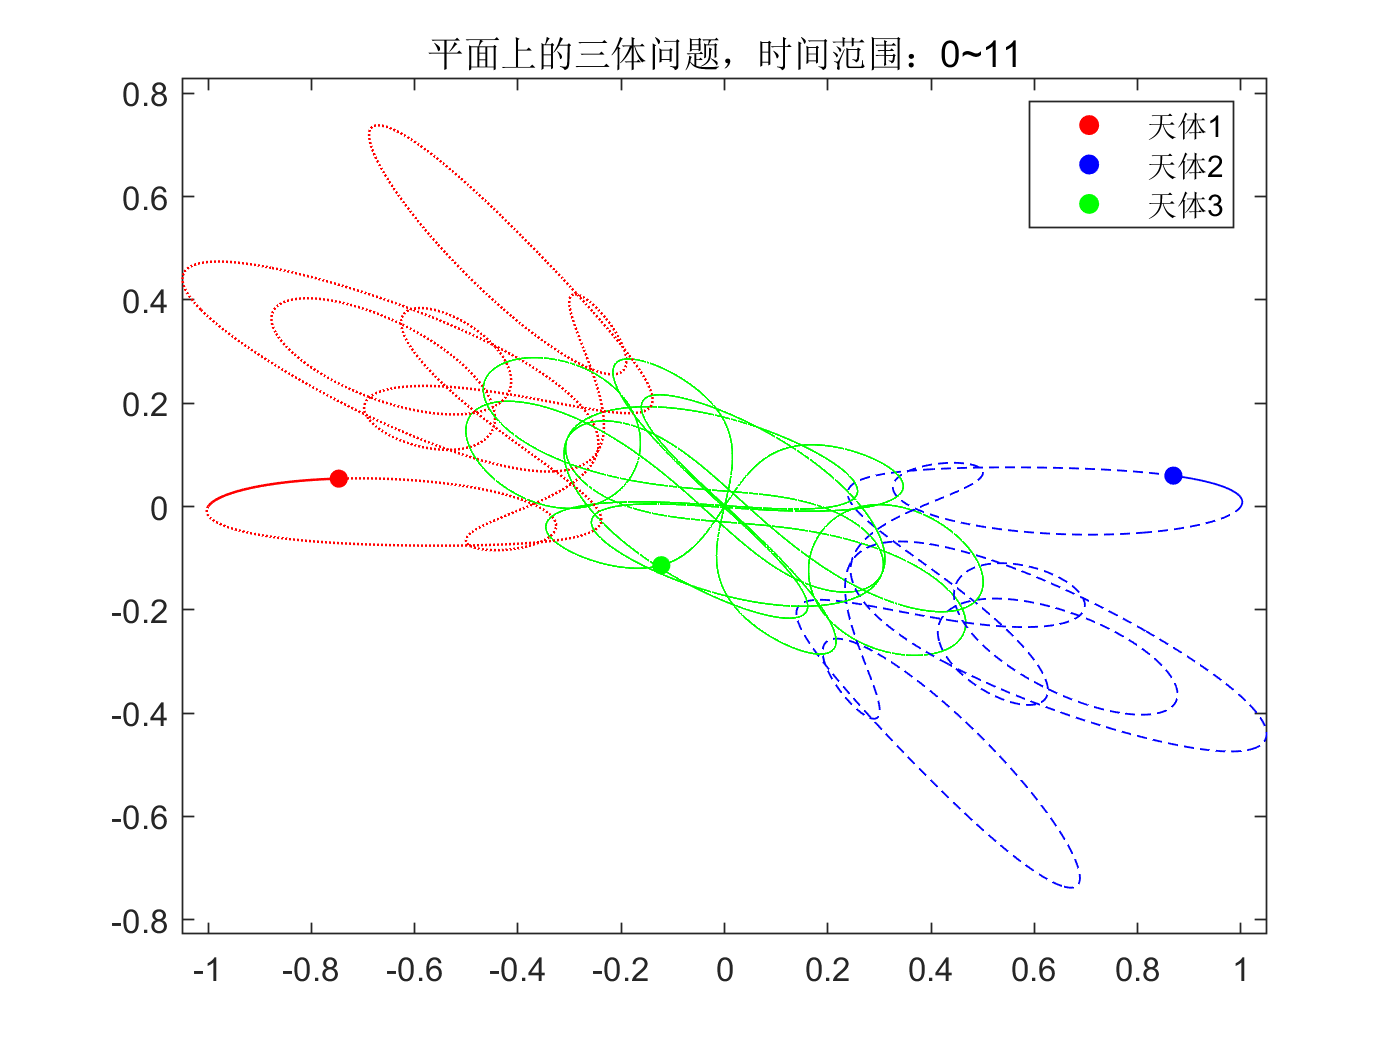
\includegraphics[width=0.7\textwidth]{一些优美的周期解//GOGGLES}
	\caption{GOGGLES的轨迹}
	\label{GOGGLES}
\end{figure}


\subsection{BUTTERFLY I}
\par
关于这个轨道的更多信息可参考\url{http://three-body.ipb.ac.rs/sol.php?id=2}
\par 初始条件如下:
\begin{align*}
	p_1& = 0.306893, p_2= 0.125507;\\
	x_1&= -1 , y_1= 0,	v_{x_1}= p_1, v_{y_1}= p_2;\\
	x_2&= 1 , y_2= 0,	v_{x_2}= p_1, v_{y_2}= p_2;\\
	x_3&= 0 ,y_3=0,		v_{x3}= -2p_1; v_{y_3}= -2p_2;
\end{align*}
\par 轨迹如下:
\begin{figure}[H]
	\centering  %图片全局居中
	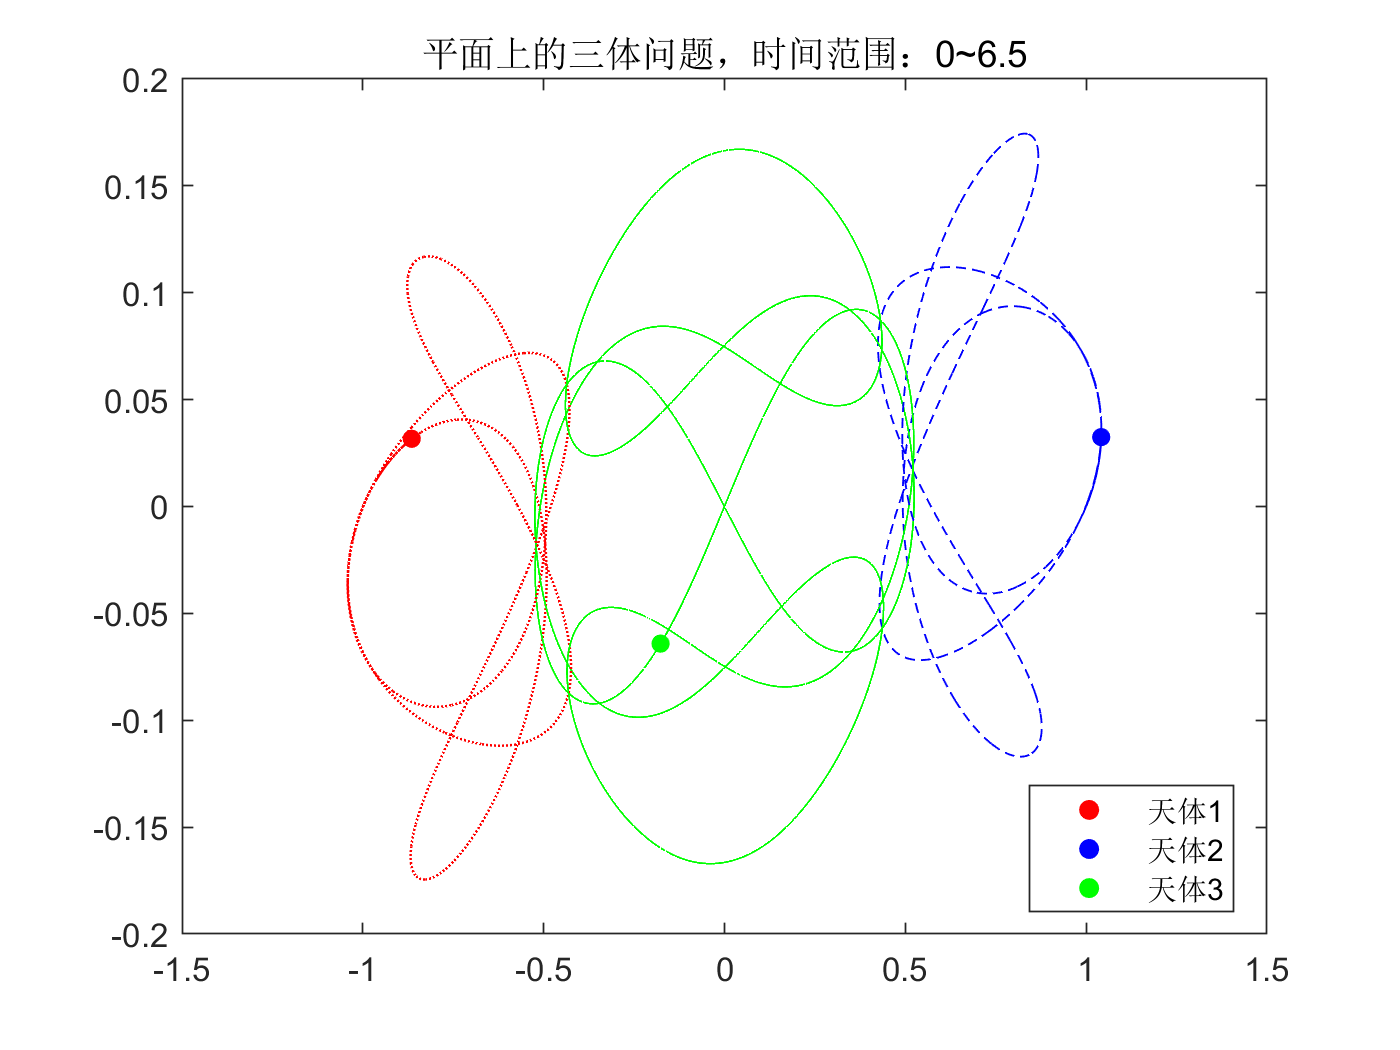
\includegraphics[width=0.7\textwidth]{一些优美的周期解//BUTTERFLY I}
	\caption{BUTTERFLY I的轨迹}
	\label{BUTTERFLY_1}
\end{figure}
\subsection{对上述不同初始条件的说明}
\par 上述的不同初始条件中,Oval,catface,and starship,GOGGLESB和BUTTERFLY I三个轨道,对数值计算的误差十分敏感,需要很小的步长(大约需要$h=\text{1e-4}$),否则会迅速突变为杂乱无章的情况,比如天体被抛射到无穷远;相比之下,Broucke R 1和Henon 35这两个轨道则只需要比较大的步长(大约$h=\text{1e-3}$),即可计算得比较准确。这也间接地说明,同样是三体问题,计算不同类型的轨道,对初值的依赖程度也是不同的。关于三体问题对初值的敏感性依赖将在下一节进行说明。
\section{N体问题的初值敏感性}
\par 下面用两个例子进一步说明N体问题对初值十分敏感。
\subsection{"8"字形轨道}
\par 第一个例子是“8”字形轨道,由C.Moore在1993年发现\cite{sauer2018数值分析},三个质量相同的天体在一个“8”字形轨道上相互追逐。其初值条件如下:
\begin{align*}
	m_1&= 1, x_1= -0.970 ,y_1= 0.243,\, v_{x_1}= -0.466, v_{y_1}= -0.433;\\
	m_2&=1,  x_2= -x_1 ,y_2= -y_1,	\, v_{x_2}=v_{x_1}  ,v_{y_2}= -v_{y_1};\\
	m_3&=1,  x_3= 0 ,y_3=0,\, v_{x_3}= -2v_{x_1}, v_{y_3}= -2v_{y_1};\\
\end{align*}
\par 三个天体的轨迹如下:
\begin{figure}[H]
	\centering  %图片全局居中
	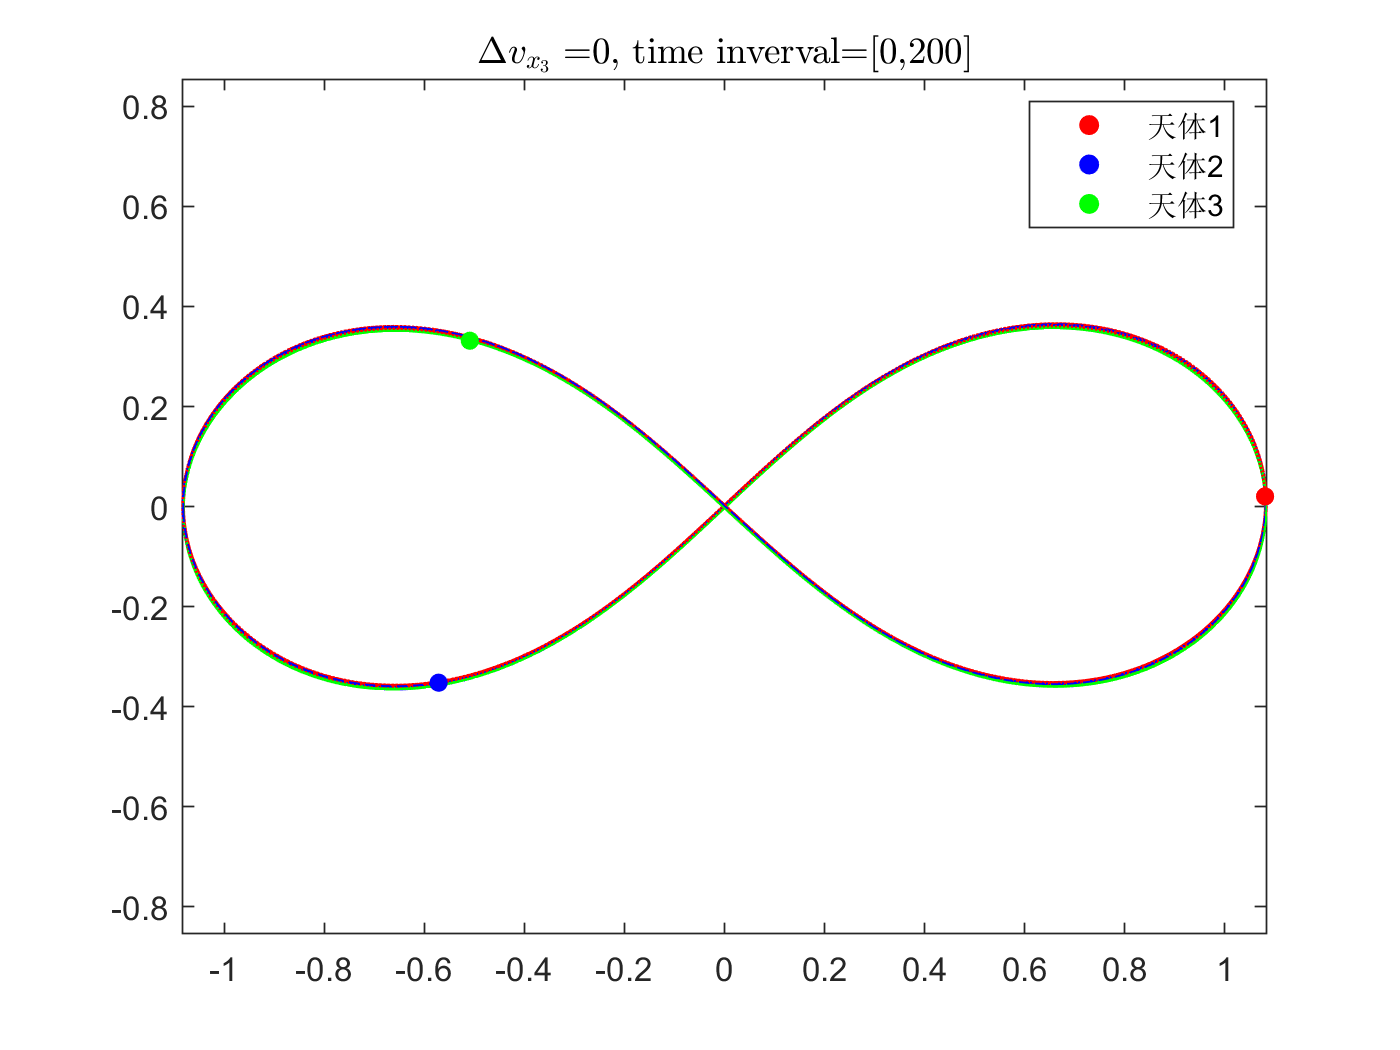
\includegraphics[width=0.7\textwidth]{八字形轨道-初值敏感1//无扰动}
	\caption{“8”字形轨道}
	\label{8_orbit}
\end{figure}
\par 对$v_{y_2}$施加扰动,即$\tilde{v_{y_2}}=v_{y_2}+\Delta v_{y_2}$,下面列出的是在$t\in[0,200]$的时间范围内,$\Delta v_{y_2}=10^{-k},\, (k=1,2,3,4)$时的轨迹突变情况。
\begin{figure}[htbp]
	\centering
	\subfigure[扰动=0.1]
	{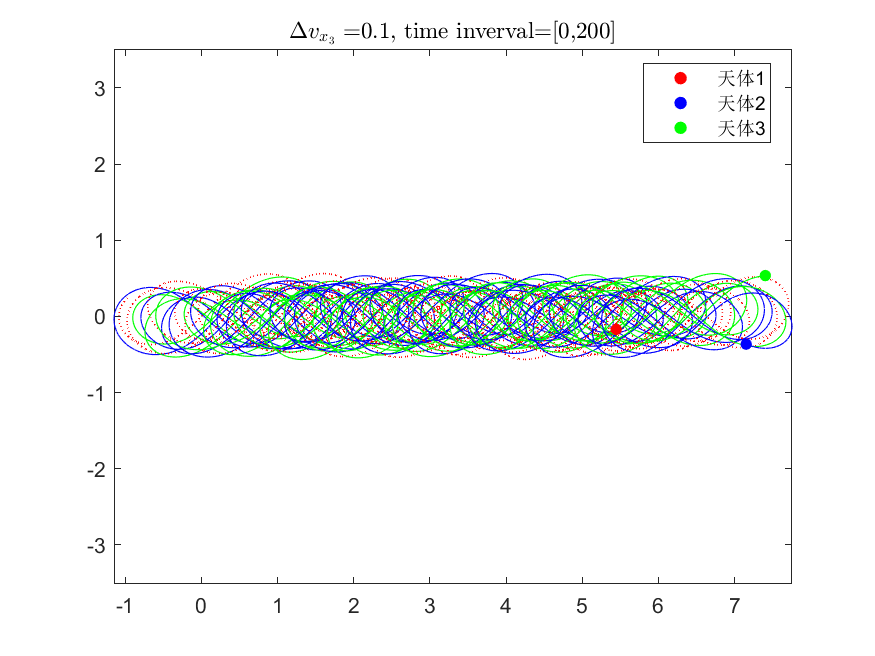
\includegraphics[width=0.45\textwidth]{八字形轨道-初值敏感1//扰动=0.1}\label{8_orbit_error_1e-1}}
	\,    % 重点就在这,优先横向排列,自动换行
	\subfigure[扰动=0.01]
	{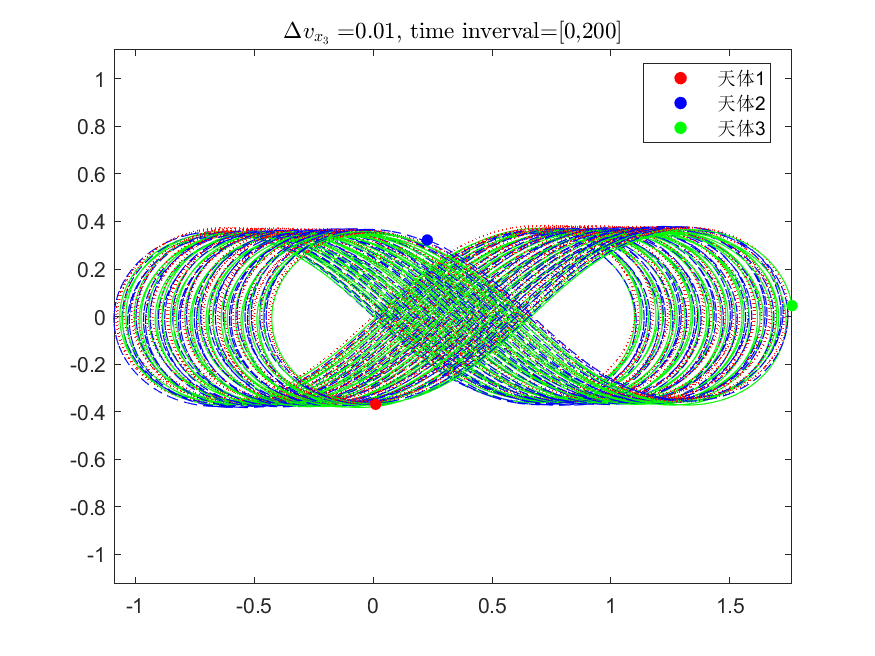
\includegraphics[width=0.45\textwidth]{八字形轨道-初值敏感1//扰动=0.01}\label{8_orbit_error_1e-2}}
	\,
	\subfigure[扰动=0.001]
	{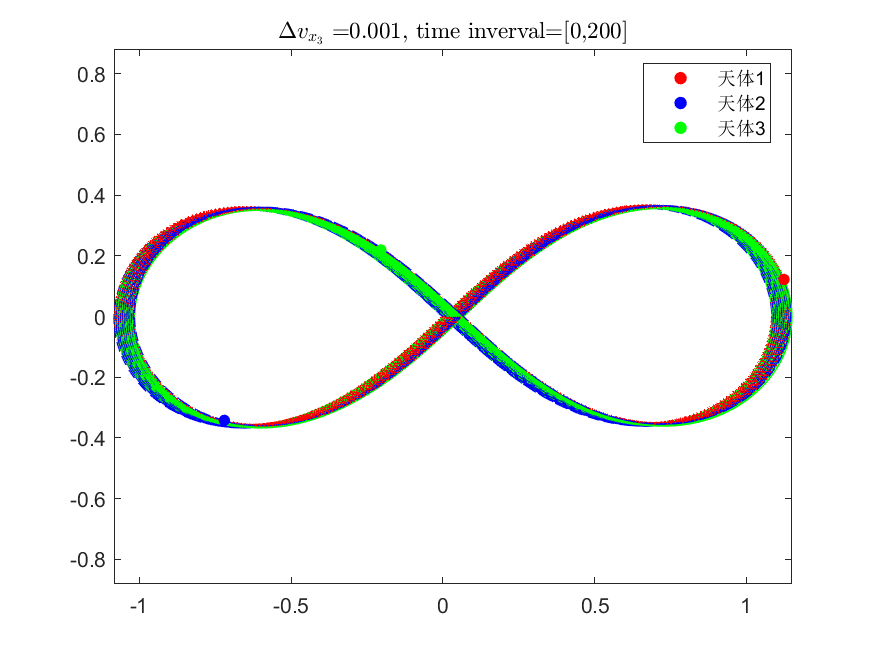
\includegraphics[width=0.45\textwidth]{八字形轨道-初值敏感1//扰动=0.001}\label{8_orbit_error_1e-3}}
	\,
	\subfigure[扰动=0.0001]
	{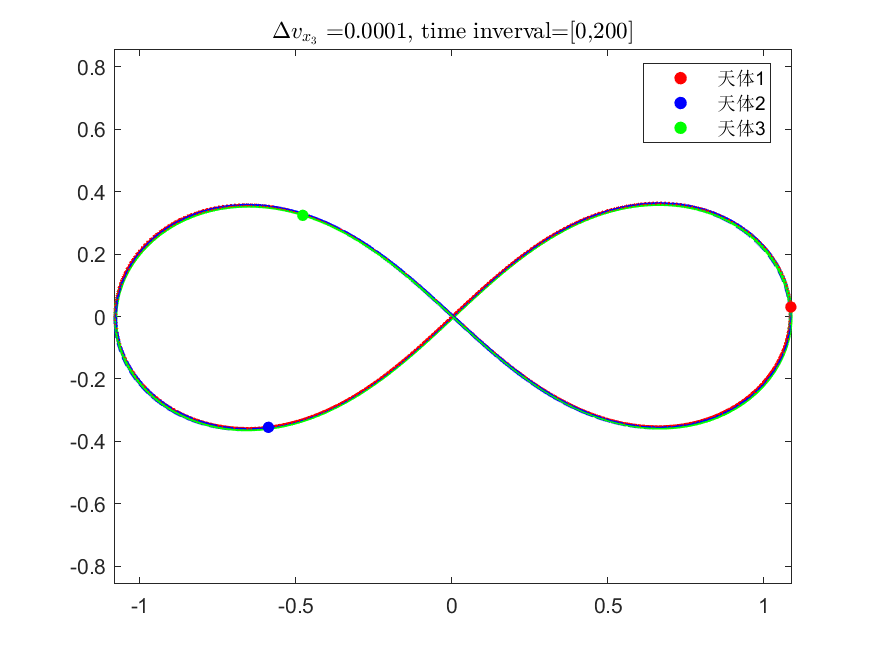
\includegraphics[width=0.45\textwidth]{八字形轨道-初值敏感1//扰动=0.0001}\label{8_orbit_error_1e-4}}
	
	\caption{"8"字形轨道的初值受到不同程度扰动后的突变情况,$t\in[0,200]$}
\end{figure}

可以看出,在$t\in[0,200]$的时间范围以内,扰动的数量级在1e-3时,已经能看出轨道趋于混沌的端倪。而扰动的数量级为1e-2时,混沌状态已经变得极其明显。
\subsection{毕达哥拉斯问题}
\par 第二个例子是毕达哥拉斯问题,这个问题最初是用来测试数值算法的。毕达哥拉斯问题取材于勾股定理,也即把质量分别为3,4,5的天体,放在边长为3,4,5的直角三角形的三个顶点上,初始速度均为零,计算其运动轨迹。具体而言,初始条件为:
\begin{align*}
	m_1&=5,x_1= 0 ,y_1= 0,v_{x_1}= 0, v_{y_1}= 0;\\
	m_2&=4,x_2= 3 ,y_2= 0,	v_{x_2}= 0 ,v_{y_2}= 0;\\
	m_3&=3,x_3= 0 ,y_3=4,v_{x_3}= 0, v_{y_3}=0;
\end{align*}
\par 毕达哥拉斯问题的最终的结果是:其中两个天体形成双星系统,而余下一个天体被抛射出去,如图\ref{BDGLS}所示:
\begin{figure}[H]
	\centering  %图片全局居中
	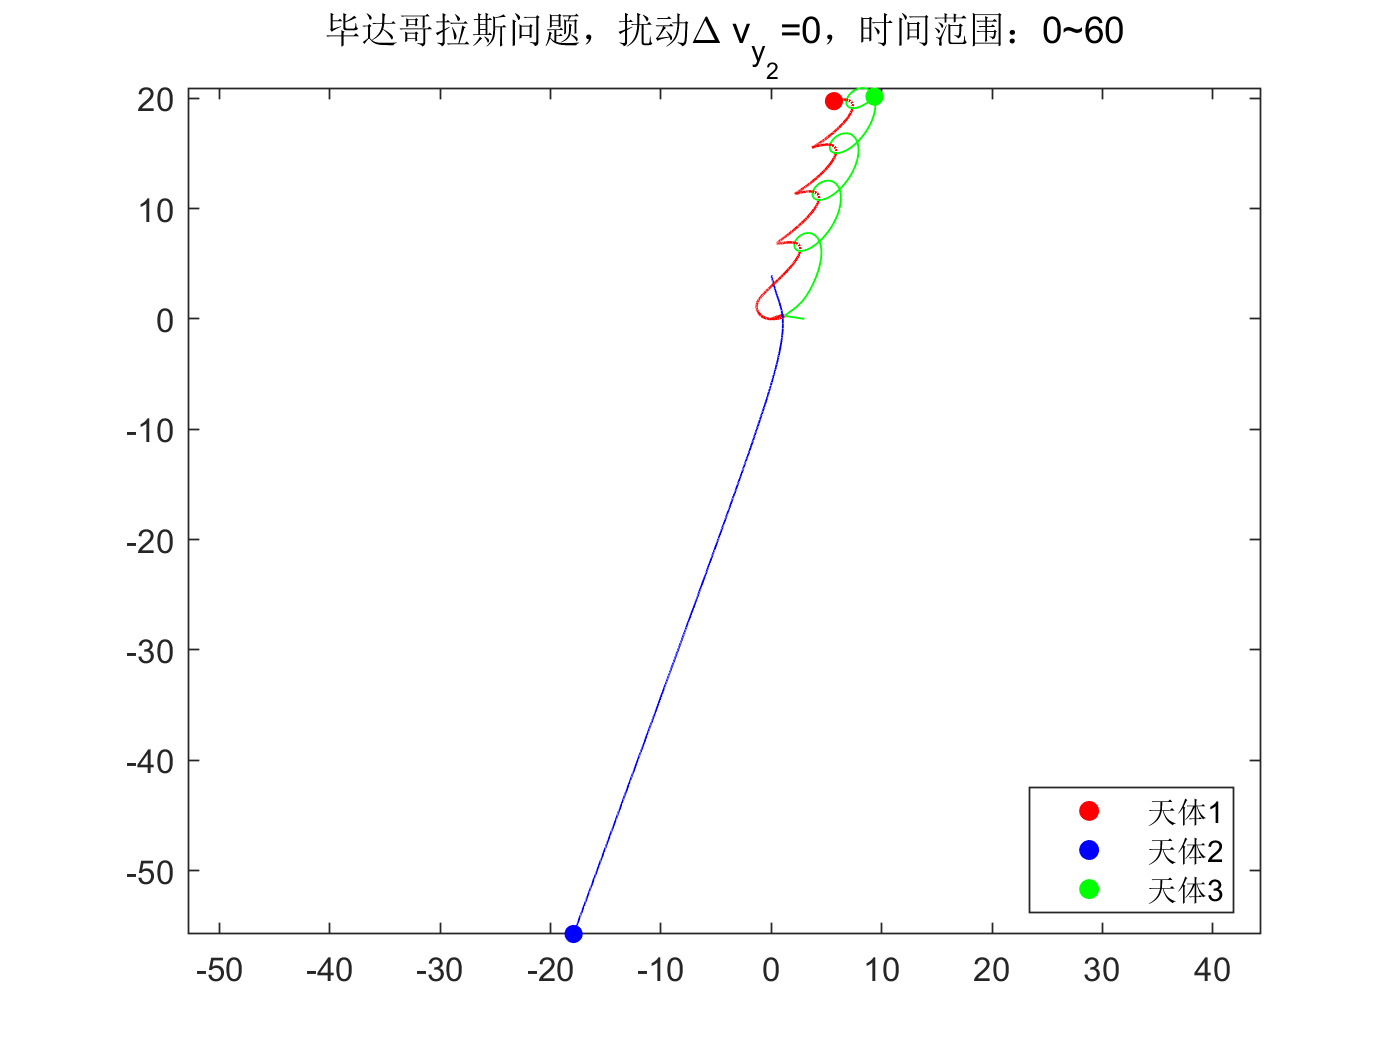
\includegraphics[width=0.7\textwidth]{毕达哥拉斯问题-初值敏感2//扰动0}
	\caption{毕达哥拉斯问题}
	\label{BDGLS}
\end{figure}
\par 现在,对第二个天体的初始y方向速度$v_{y_2}$施加扰动,即$\tilde{v_{y_2}}=\Delta v_{y_2}$,图\ref{BDGLS_error}分别展示了$\Delta v_{y_2} = 10^{-k},\, (k=3,4)$时,轨迹发生的明显突变。
\begin{figure}[H]
	\centering  %图片全局居中
	\subfigure[扰动=1e-3]{
		\label{BDGLS_error_1e-3}
		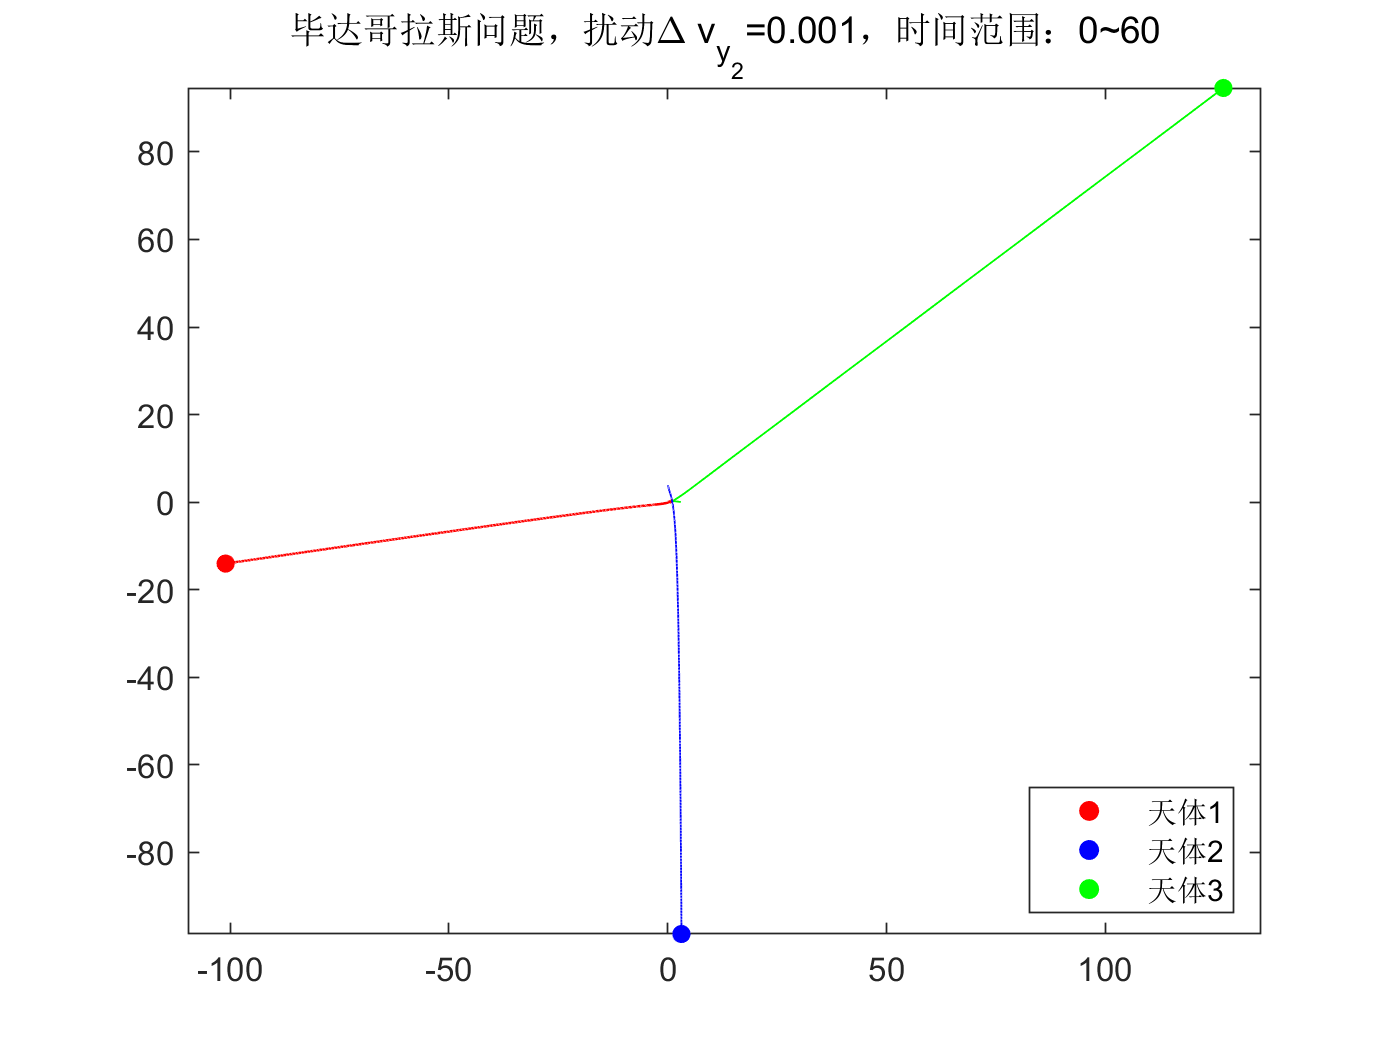
\includegraphics[width=0.45\textwidth]{毕达哥拉斯问题-初值敏感2//扰动1e-3}}
	\subfigure[扰动=1e-4]{
		\label{BDGLS_error_1e-4}
		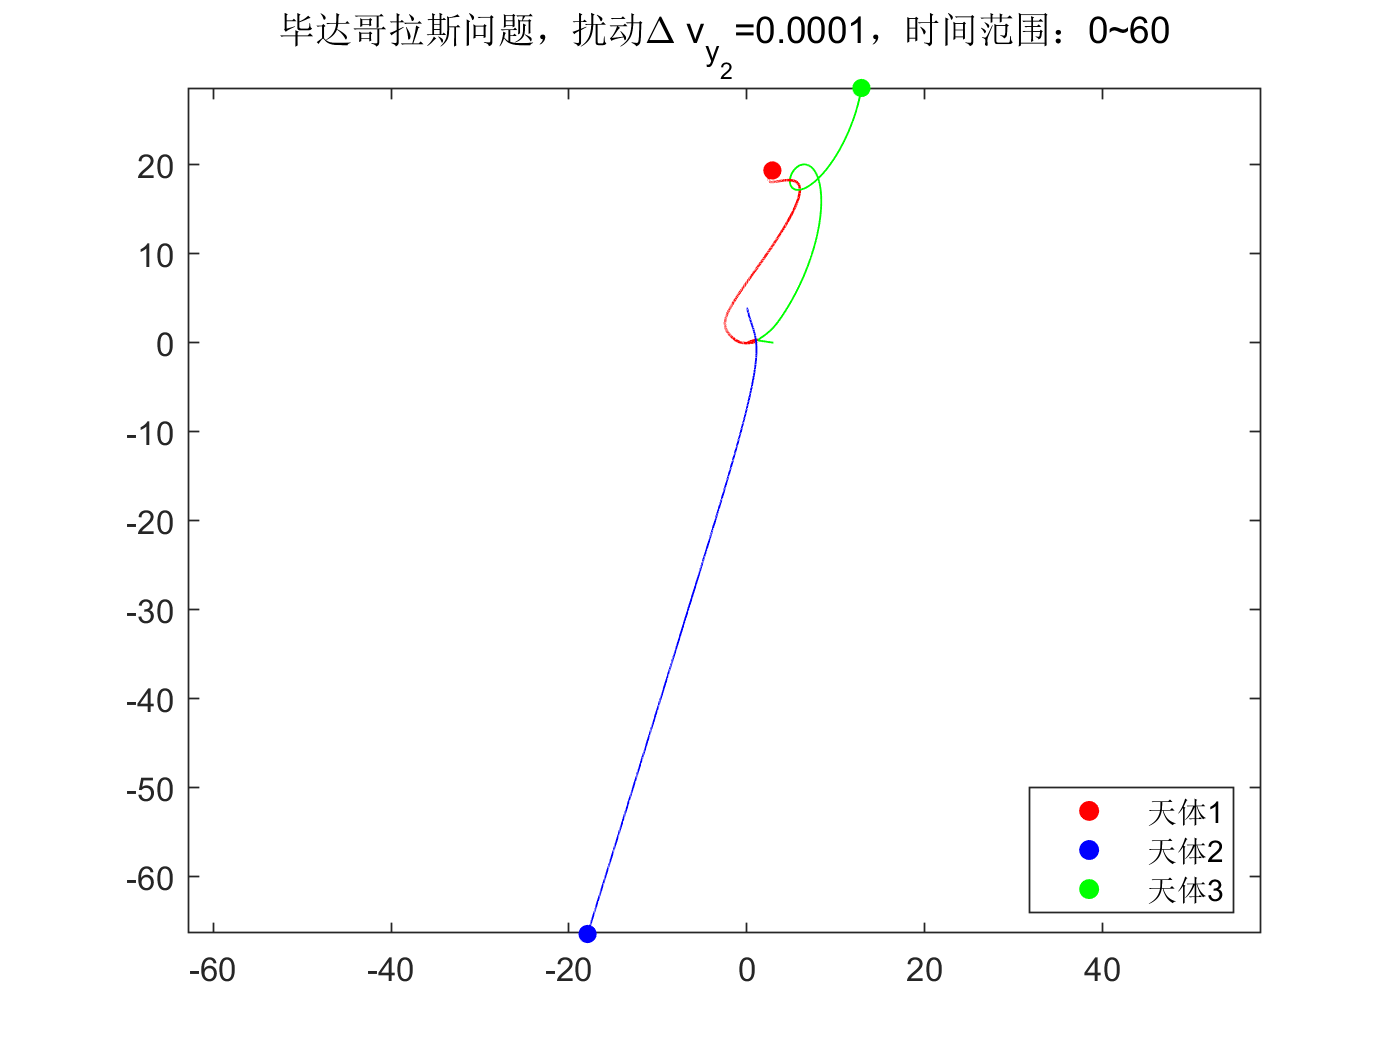
\includegraphics[width=0.45\textwidth]{毕达哥拉斯问题-初值敏感2//扰动1e-4}}
	\caption{毕达哥拉斯问题的初值受到不同程度的扰动后的轨迹突变情况}
	\label{BDGLS_error}
\end{figure}

\section{拉格朗日点}
\par 当第三个天体的质量可以忽略时,例如在“太阳-地球-人造卫星”系统中,三体问题则变为“限制性三体问题”,可以直接在建模过程中设置$m_3=0$,而微分方程组的形式不发生变化,那么,该问题依然可以用同样的数值方法进行模拟。
\par 在“限制性三体问题”中,我们仍然关心稳定的周期性轨道。其中一类相当有实际意义的轨道,就是第三个天体恰好处于拉格朗日点时的三体运动轨迹。当第三个天体处于拉格朗日点时,其受到其他两个天体的引力之合力恰好作为其进行圆周运动的向心力,此时三个天体将具有相同的角速度。
\par 前三个拉格朗日点L1,L2,L3比较出名,分别在两个天体连线上以及延长线上,很多的人造卫星和天文望远镜,常常发送到这些点附近。而L4和L5则比较特殊,分别处于前两个天体连线的双侧,并且使得三个天体之间距离相等,构成等边三角形(请参考\url{https://zhuanlan.zhihu.com/p/339028468})。比如在“太阳-木星”系统中,就观测到聚集在L4和L5附近的特洛伊小行星群,一部分运行在木星之前,一部分跟随在木星之后。
\par 本文以L4拉格朗日点为例进行实验,初始条件为:
\begin{align*}
	m_1&=3,x_1= -1 ,y_1= 0,v_{x_1}= 0, v_{y_1}= -0.25;\\
	m_2&=1,x_2= 3 ,y_2= 0,	v_{x_2}= 0 ,v_{y_2}= 0.75;\\
	m_3&=0,x_3= 1 ,y_3=2 \sqrt{3},v_{x_3}= -\frac{\sqrt{3}}{2}, v_{y_3}=0.25;
\end{align*}
\par 三个天体初始位置如下图\ref{Lagrange_init}所示:
\begin{figure}[H]
	\centering  %图片全局居中
	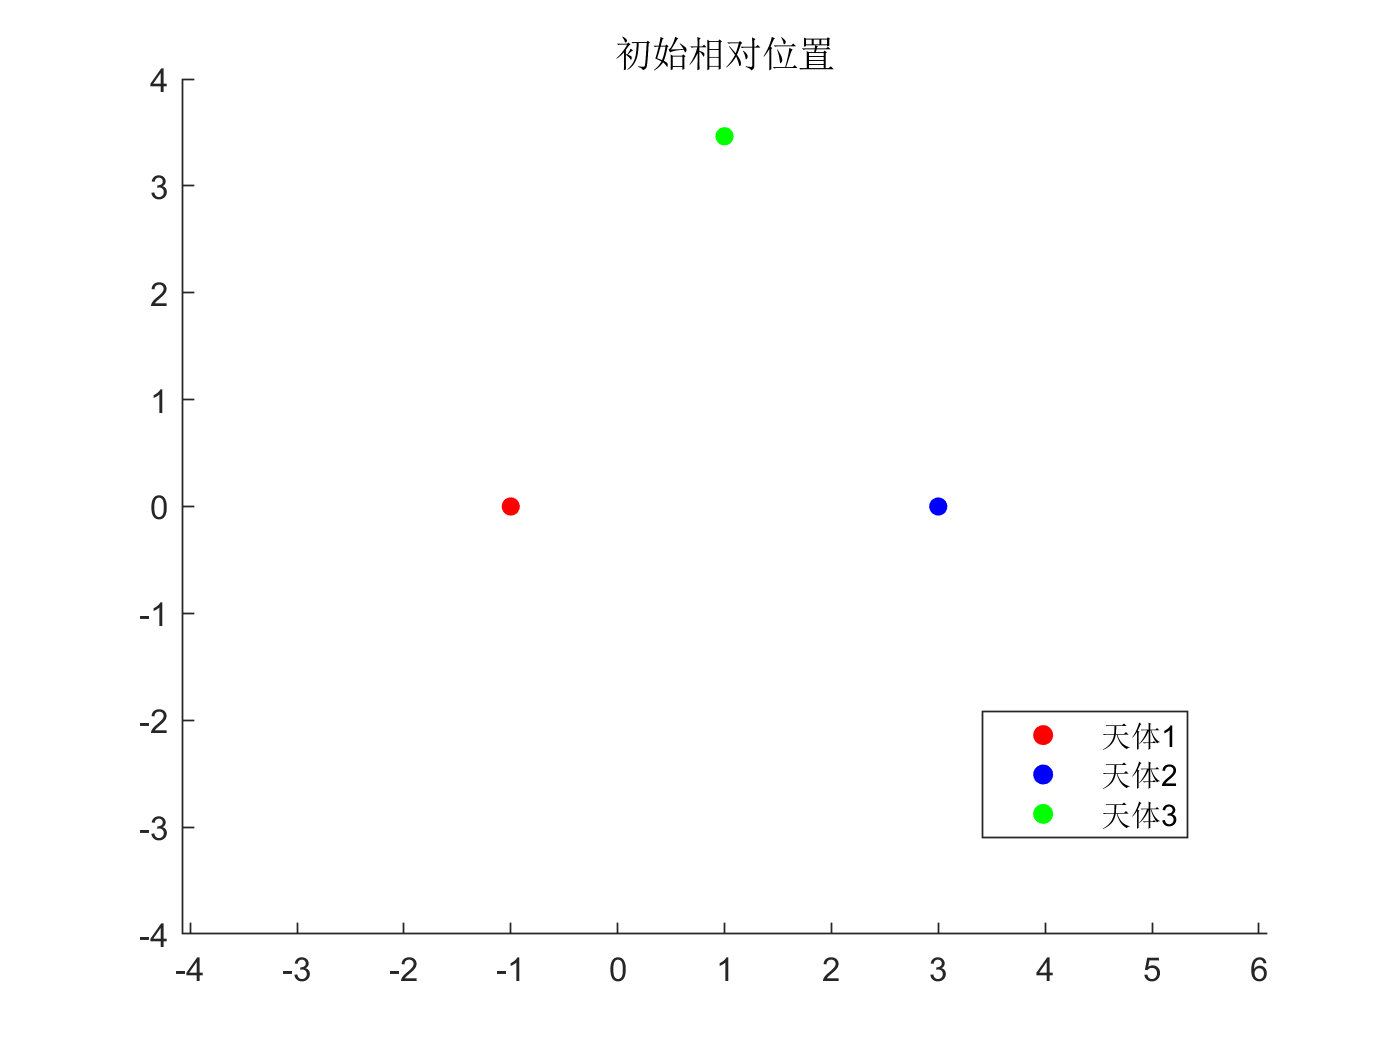
\includegraphics[width=0.7\textwidth]{拉格朗日点L4//拉格朗日点 初始状态}
	\caption{L4拉格朗日点数值模拟的初始位置状态}
	\label{Lagrange_init}
\end{figure}

\par 实验结果如下:
\begin{figure}[H]
	\centering  %图片全局居中
	\subfigure[截至时间t=22]{
		\label{lagrange_22}
		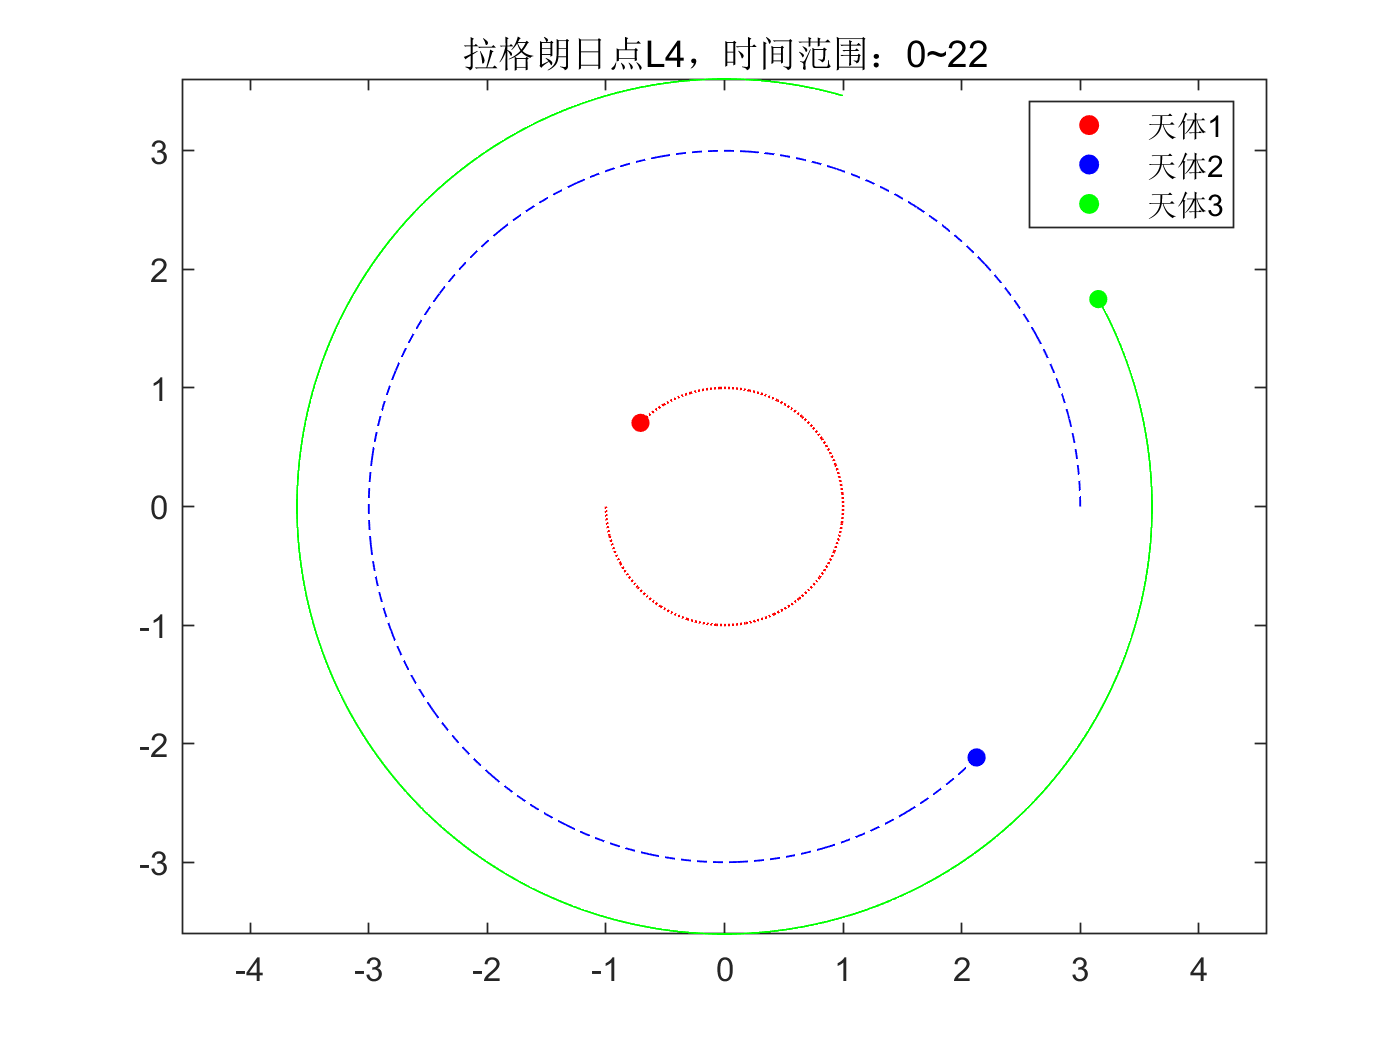
\includegraphics[width=0.45\textwidth]{拉格朗日点L4//拉格朗日点 0~22}}
	\subfigure[截至时间t=100]{
		\label{lagrange_100}
		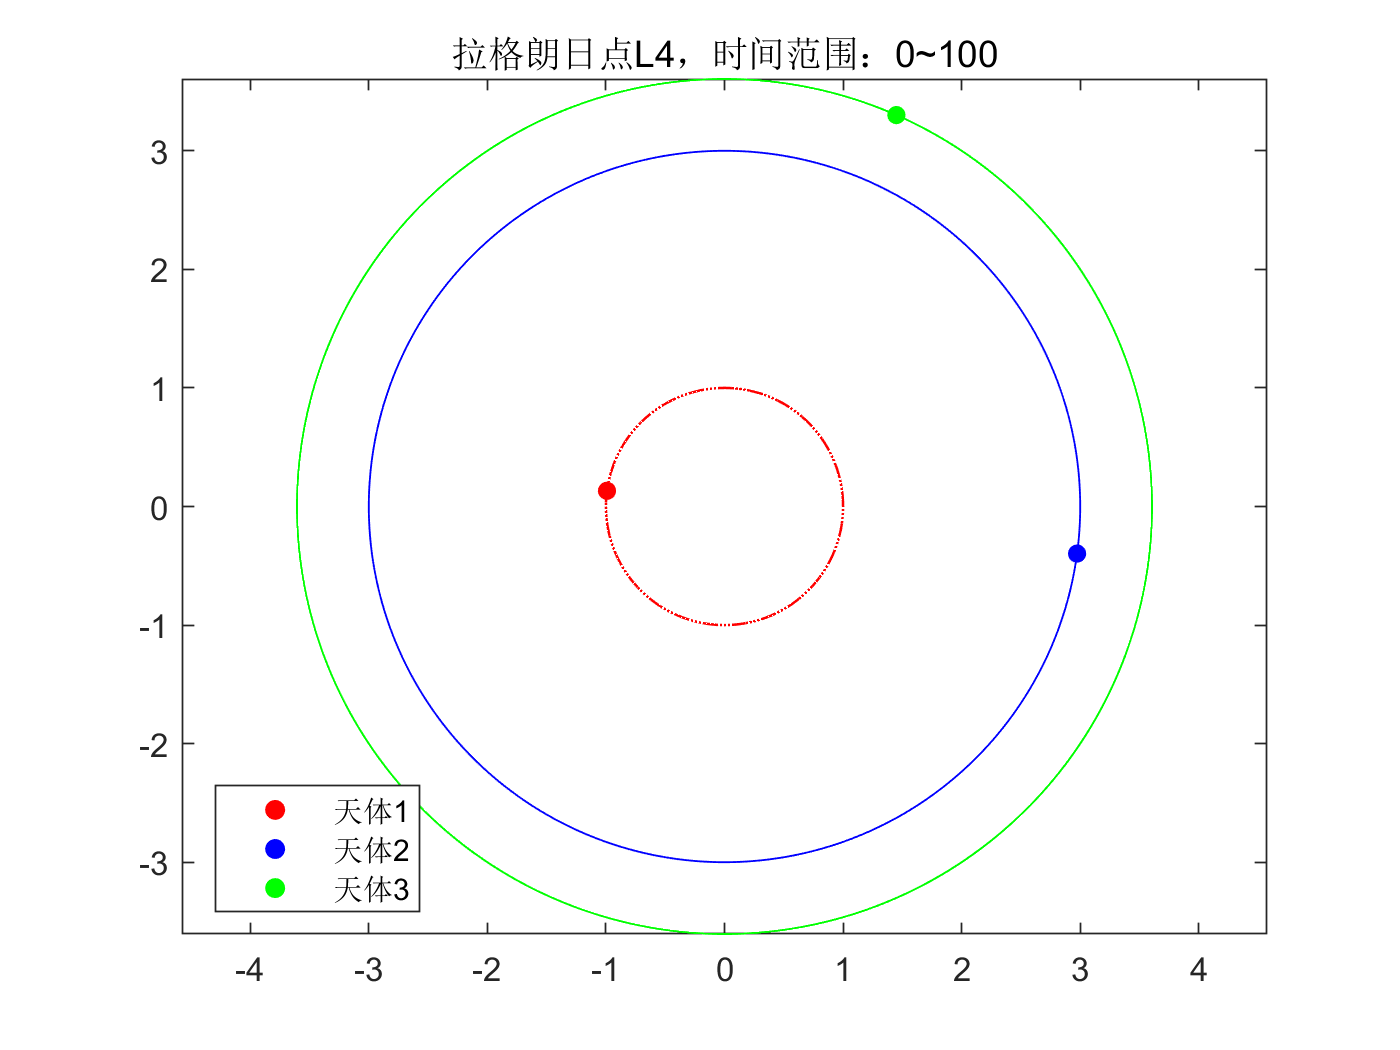
\includegraphics[width=0.45\textwidth]{拉格朗日点L4//拉格朗日点 0~100}}
	\caption{第三个天体处于L4拉格朗日点时的运行轨迹}
	\label{lagrange}
\end{figure}
\par 可以看出,三个天体之间确实能够保持等边三角形的相对位置,并且各自运行在所属圆轨道上,十分稳定。
\section{报告小结}
\par 本文探究了平面上的单体问题、二体问题、三体问题和限制性三体问题,比较了不同数值方法在求解N体问题上的优劣,展示了一些具有代表性的三体问题周期性轨迹,用实例说明了N体问题对初值极端敏感的依赖性,并展示了在限制性三体问题中小质量卫星处于L4拉格朗日点时的稳定运动轨迹。
\par 本研究尚存不足之处包括:缺乏对不同数值方法在解决N体问题之优劣的理论分析,没有对稳定三体问题周期性轨迹所满足的初值条件做进一步的探究。希望在未来的有关课程中,对上述问题做更深入探究。
\bibliographystyle{unsrt}
\bibliography{ref.bib}
\end{document}